\documentclass[twoside]{book}

% Packages required by doxygen
\usepackage{fixltx2e}
\usepackage{calc}
\usepackage{doxygen}
\usepackage[export]{adjustbox} % also loads graphicx
\usepackage{graphicx}
\usepackage[utf8]{inputenc}
\usepackage{makeidx}
\usepackage{multicol}
\usepackage{multirow}
\PassOptionsToPackage{warn}{textcomp}
\usepackage{textcomp}
\usepackage[nointegrals]{wasysym}
\usepackage[table]{xcolor}

% Font selection
\usepackage[T1]{fontenc}
\usepackage[scaled=.90]{helvet}
\usepackage{courier}
\usepackage{amssymb}
\usepackage{sectsty}
\renewcommand{\familydefault}{\sfdefault}
\allsectionsfont{%
  \fontseries{bc}\selectfont%
  \color{darkgray}%
}
\renewcommand{\DoxyLabelFont}{%
  \fontseries{bc}\selectfont%
  \color{darkgray}%
}
\newcommand{\+}{\discretionary{\mbox{\scriptsize$\hookleftarrow$}}{}{}}

% Page & text layout
\usepackage{geometry}
\geometry{%
  a4paper,%
  top=2.5cm,%
  bottom=2.5cm,%
  left=2.5cm,%
  right=2.5cm%
}
\tolerance=750
\hfuzz=15pt
\hbadness=750
\setlength{\emergencystretch}{15pt}
\setlength{\parindent}{0cm}
\setlength{\parskip}{3ex plus 2ex minus 2ex}
\makeatletter
\renewcommand{\paragraph}{%
  \@startsection{paragraph}{4}{0ex}{-1.0ex}{1.0ex}{%
    \normalfont\normalsize\bfseries\SS@parafont%
  }%
}
\renewcommand{\subparagraph}{%
  \@startsection{subparagraph}{5}{0ex}{-1.0ex}{1.0ex}{%
    \normalfont\normalsize\bfseries\SS@subparafont%
  }%
}
\makeatother

% Headers & footers
\usepackage{fancyhdr}
\pagestyle{fancyplain}
\fancyhead[LE]{\fancyplain{}{\bfseries\thepage}}
\fancyhead[CE]{\fancyplain{}{}}
\fancyhead[RE]{\fancyplain{}{\bfseries\leftmark}}
\fancyhead[LO]{\fancyplain{}{\bfseries\rightmark}}
\fancyhead[CO]{\fancyplain{}{}}
\fancyhead[RO]{\fancyplain{}{\bfseries\thepage}}
\fancyfoot[LE]{\fancyplain{}{}}
\fancyfoot[CE]{\fancyplain{}{}}
\fancyfoot[RE]{\fancyplain{}{\bfseries\scriptsize Generated by Doxygen }}
\fancyfoot[LO]{\fancyplain{}{\bfseries\scriptsize Generated by Doxygen }}
\fancyfoot[CO]{\fancyplain{}{}}
\fancyfoot[RO]{\fancyplain{}{}}
\renewcommand{\footrulewidth}{0.4pt}
\renewcommand{\chaptermark}[1]{%
  \markboth{#1}{}%
}
\renewcommand{\sectionmark}[1]{%
  \markright{\thesection\ #1}%
}

% Indices & bibliography
\usepackage{natbib}
\usepackage[titles]{tocloft}
\setcounter{tocdepth}{3}
\setcounter{secnumdepth}{5}
\makeindex

% Hyperlinks (required, but should be loaded last)
\usepackage{ifpdf}
\ifpdf
  \usepackage[pdftex,pagebackref=true]{hyperref}
\else
  \usepackage[ps2pdf,pagebackref=true]{hyperref}
\fi
\hypersetup{%
  colorlinks=true,%
  linkcolor=blue,%
  citecolor=blue,%
  unicode%
}

% Custom commands
\newcommand{\clearemptydoublepage}{%
  \newpage{\pagestyle{empty}\cleardoublepage}%
}

\usepackage{caption}
\captionsetup{labelsep=space,justification=centering,font={bf},singlelinecheck=off,skip=4pt,position=top}

%===== C O N T E N T S =====

\begin{document}

% Titlepage & ToC
\hypersetup{pageanchor=false,
             bookmarksnumbered=true,
             pdfencoding=unicode
            }
\pagenumbering{roman}
\begin{titlepage}
\vspace*{7cm}
\begin{center}%
{\Large Voyager\+: Exploratpry robot }\\
\vspace*{1cm}
{\large Generated by Doxygen 1.8.11}\\
\end{center}
\end{titlepage}
\clearemptydoublepage
\tableofcontents
\clearemptydoublepage
\pagenumbering{arabic}
\hypersetup{pageanchor=true}

%--- Begin generated contents ---
\chapter{Voyager\+: Explore the environment!}
\label{md__home_nrparikh_hector_quadrotor_tutorial_src_voyager_README}
\hypertarget{md__home_nrparikh_hector_quadrotor_tutorial_src_voyager_README}{}
\href{https://travis-ci.org/nr-parikh/voyager}{\tt } \href{https://github.com/nr-parikh/voyager/blob/master/LICENSE}{\tt }

Voyager\+: Exploratory robot which performs S\+L\+AM in the environment.

The S\+IP for the project can be found \href{https://docs.google.com/spreadsheets/d/11tZz-o4cJSky1bMGR0uIQGLcoGgMJUM74vtqE4XKSQ8/edit?usp=sharing}{\tt here}.

Planning notes can be found \href{https://docs.google.com/document/d/1XSsnkajWHP6XwBxO1Zjkb_wmKyFWa5k23H9Gzb1IpiQ/edit?usp=sharing}{\tt here}.

\subsection*{First sprint update}

Things done in the first sprint\+: \begin{DoxyVerb}* Install all the packages necessary to run **hector** quadrotor package.
* Test the working of the necessary packages and check the data being received from the robot
* Explore various SLAM packages that can be used in this project
* Create initial UML diagrams
* Setup Travis for the repository
* Create SIP log
\end{DoxyVerb}


\subsection*{Second sprint update}

Things done in second sprint\+: \begin{DoxyVerb}* Create a custom gazebo world that can be used a testing rig to test the performance of the algorithm 
* Create stub implementation of the classes 
* Create isAlive test cases for the classes 
* Search how to integrate OctoMap wit hector_slam 
* Try to improve the results of rgbdslam 
* Control the quadrotor using commandline as well as dummy script.
* Create planning notes and update SIP tasklog as well as release backlog.  \end{DoxyVerb}
 
\chapter{Class Index}
\section{Class List}
Here are the classes, structs, unions and interfaces with brief descriptions\+:\begin{DoxyCompactList}
\item\contentsline{section}{\hyperlink{class_laser_scan}{Laser\+Scan} }{\pageref{class_laser_scan}}{}
\item\contentsline{section}{\hyperlink{class_planner}{Planner} }{\pageref{class_planner}}{}
\item\contentsline{section}{\hyperlink{class_quadrotor}{Quadrotor} }{\pageref{class_quadrotor}}{}
\end{DoxyCompactList}

\chapter{File Index}
\section{File List}
Here is a list of all files with brief descriptions\+:\begin{DoxyCompactList}
\item\contentsline{section}{/home/nrparikh/hector\+\_\+quadrotor\+\_\+tutorial/src/voyager/include/voyager/\hyperlink{laser__scan_8hpp}{laser\+\_\+scan.\+hpp} \\*D\+E\+S\+C\+R\+I\+P\+T\+I\+ON Header file for the class \hyperlink{class_laser_scan}{Laser\+Scan} }{\pageref{laser__scan_8hpp}}{}
\item\contentsline{section}{/home/nrparikh/hector\+\_\+quadrotor\+\_\+tutorial/src/voyager/include/voyager/\hyperlink{planner_8hpp}{planner.\+hpp} \\*D\+E\+S\+C\+R\+I\+P\+T\+I\+ON Header file for the class \hyperlink{class_planner}{Planner} }{\pageref{planner_8hpp}}{}
\item\contentsline{section}{/home/nrparikh/hector\+\_\+quadrotor\+\_\+tutorial/src/voyager/include/voyager/\hyperlink{quadrotor_8hpp}{quadrotor.\+hpp} \\*D\+E\+S\+C\+R\+I\+P\+T\+I\+ON Header file for the classs \hyperlink{class_quadrotor}{Quadrotor} }{\pageref{quadrotor_8hpp}}{}
\item\contentsline{section}{/home/nrparikh/hector\+\_\+quadrotor\+\_\+tutorial/src/voyager/src/\hyperlink{laser__scan_8cpp}{laser\+\_\+scan.\+cpp} \\*D\+E\+S\+C\+R\+I\+P\+T\+I\+ON Class implementation for the class \hyperlink{class_laser_scan}{Laser\+Scan} }{\pageref{laser__scan_8cpp}}{}
\item\contentsline{section}{/home/nrparikh/hector\+\_\+quadrotor\+\_\+tutorial/src/voyager/src/\hyperlink{planner_8cpp}{planner.\+cpp} \\*D\+E\+S\+C\+R\+I\+P\+T\+I\+ON Implementation of the class \hyperlink{class_planner}{Planner} }{\pageref{planner_8cpp}}{}
\item\contentsline{section}{/home/nrparikh/hector\+\_\+quadrotor\+\_\+tutorial/src/voyager/src/\hyperlink{quadrotor_8cpp}{quadrotor.\+cpp} \\*D\+E\+S\+C\+R\+I\+P\+T\+I\+ON Implementation of the class \hyperlink{class_quadrotor}{Quadrotor} }{\pageref{quadrotor_8cpp}}{}
\item\contentsline{section}{/home/nrparikh/hector\+\_\+quadrotor\+\_\+tutorial/src/voyager/src/\hyperlink{voyager_8cpp}{voyager.\+cpp} \\*D\+E\+S\+C\+R\+I\+P\+T\+I\+ON Main file for the package voyager }{\pageref{voyager_8cpp}}{}
\item\contentsline{section}{/home/nrparikh/hector\+\_\+quadrotor\+\_\+tutorial/src/voyager/test/\hyperlink{test__laser__scan_8cpp}{test\+\_\+laser\+\_\+scan.\+cpp} \\*D\+E\+S\+C\+R\+I\+P\+T\+I\+ON Unit tests for the class \hyperlink{class_laser_scan}{Laser\+Scan} }{\pageref{test__laser__scan_8cpp}}{}
\item\contentsline{section}{/home/nrparikh/hector\+\_\+quadrotor\+\_\+tutorial/src/voyager/test/\hyperlink{test__planner_8cpp}{test\+\_\+planner.\+cpp} \\*D\+E\+S\+C\+R\+I\+P\+T\+I\+ON Unit tests for the class \hyperlink{class_planner}{Planner} }{\pageref{test__planner_8cpp}}{}
\item\contentsline{section}{/home/nrparikh/hector\+\_\+quadrotor\+\_\+tutorial/src/voyager/test/\hyperlink{test__quadrotor_8cpp}{test\+\_\+quadrotor.\+cpp} }{\pageref{test__quadrotor_8cpp}}{}
\item\contentsline{section}{/home/nrparikh/hector\+\_\+quadrotor\+\_\+tutorial/src/voyager/test/\hyperlink{test__voyager_8cpp}{test\+\_\+voyager.\+cpp} \\*D\+E\+S\+C\+R\+I\+P\+T\+I\+ON Test file for checking the service }{\pageref{test__voyager_8cpp}}{}
\item\contentsline{section}{/home/nrparikh/hector\+\_\+quadrotor\+\_\+tutorial/src/voyager/test/\hyperlink{test__voyager__node_8cpp}{test\+\_\+voyager\+\_\+node.\+cpp} \\*D\+E\+S\+C\+R\+I\+P\+T\+I\+ON Unit tests for the package Voyager }{\pageref{test__voyager__node_8cpp}}{}
\end{DoxyCompactList}

\chapter{Class Documentation}
\hypertarget{class_laser_scan}{}\section{Laser\+Scan Class Reference}
\label{class_laser_scan}\index{Laser\+Scan@{Laser\+Scan}}


{\ttfamily \#include $<$laser\+\_\+scan.\+hpp$>$}

\subsection*{Public Member Functions}
\begin{DoxyCompactItemize}
\item 
\hyperlink{class_laser_scan_ae1c29cf38fcdf0c649691b8c609e5ce7}{Laser\+Scan} ()
\begin{DoxyCompactList}\small\item\em Constructor of the class. \end{DoxyCompactList}\item 
\hyperlink{class_laser_scan_adab7acdb2d59acb2350a1e4d93981b8a}{$\sim$\+Laser\+Scan} ()
\begin{DoxyCompactList}\small\item\em Destructor of the class. \end{DoxyCompactList}\item 
auto \hyperlink{class_laser_scan_a5550d5c98d7456d6f90fd34bda650cde}{scan\+Callback} (const sensor\+\_\+msgs\+::\+Laser\+Scan scan\+\_\+msg) -\/$>$ void
\begin{DoxyCompactList}\small\item\em Callback function. \end{DoxyCompactList}\item 
auto \hyperlink{class_laser_scan_aab0d1a864bf9d96a0396f1235d327dbd}{is\+Alive} () -\/$>$ bool
\begin{DoxyCompactList}\small\item\em Check if running. \end{DoxyCompactList}\item 
auto \hyperlink{class_laser_scan_ac86a1b1d140a88c4f4f47aaddc6de798}{check\+Collision} () -\/$>$ bool
\begin{DoxyCompactList}\small\item\em Return the obstacle flag. \end{DoxyCompactList}\end{DoxyCompactItemize}


\subsection{Detailed Description}


Definition at line 40 of file laser\+\_\+scan.\+hpp.



\subsection{Constructor \& Destructor Documentation}
\index{Laser\+Scan@{Laser\+Scan}!Laser\+Scan@{Laser\+Scan}}
\index{Laser\+Scan@{Laser\+Scan}!Laser\+Scan@{Laser\+Scan}}
\subsubsection[{\texorpdfstring{Laser\+Scan()}{LaserScan()}}]{\setlength{\rightskip}{0pt plus 5cm}Laser\+Scan\+::\+Laser\+Scan (
\begin{DoxyParamCaption}
{}
\end{DoxyParamCaption}
)}\hypertarget{class_laser_scan_ae1c29cf38fcdf0c649691b8c609e5ce7}{}\label{class_laser_scan_ae1c29cf38fcdf0c649691b8c609e5ce7}


Constructor of the class. 

Initialize node handle as well as set is\+\_\+running\+\_\+ flag to true 

Definition at line 37 of file laser\+\_\+scan.\+cpp.

\index{Laser\+Scan@{Laser\+Scan}!````~Laser\+Scan@{$\sim$\+Laser\+Scan}}
\index{````~Laser\+Scan@{$\sim$\+Laser\+Scan}!Laser\+Scan@{Laser\+Scan}}
\subsubsection[{\texorpdfstring{$\sim$\+Laser\+Scan()}{~LaserScan()}}]{\setlength{\rightskip}{0pt plus 5cm}Laser\+Scan\+::$\sim$\+Laser\+Scan (
\begin{DoxyParamCaption}
{}
\end{DoxyParamCaption}
)}\hypertarget{class_laser_scan_adab7acdb2d59acb2350a1e4d93981b8a}{}\label{class_laser_scan_adab7acdb2d59acb2350a1e4d93981b8a}


Destructor of the class. 

Write actions that needs to be done when destroying the object 

Definition at line 47 of file laser\+\_\+scan.\+cpp.



\subsection{Member Function Documentation}
\index{Laser\+Scan@{Laser\+Scan}!check\+Collision@{check\+Collision}}
\index{check\+Collision@{check\+Collision}!Laser\+Scan@{Laser\+Scan}}
\subsubsection[{\texorpdfstring{check\+Collision() -\/$>$ bool}{checkCollision() -> bool}}]{\setlength{\rightskip}{0pt plus 5cm}auto Laser\+Scan\+::check\+Collision (
\begin{DoxyParamCaption}
{}
\end{DoxyParamCaption}
) -\/$>$ bool}\hypertarget{class_laser_scan_ac86a1b1d140a88c4f4f47aaddc6de798}{}\label{class_laser_scan_ac86a1b1d140a88c4f4f47aaddc6de798}


Return the obstacle flag. 

Return true if the obstacle is present, false otherwise \begin{DoxyReturn}{Returns}
bool\+: Return the value of flag 
\end{DoxyReturn}


Definition at line 87 of file laser\+\_\+scan.\+cpp.

\index{Laser\+Scan@{Laser\+Scan}!is\+Alive@{is\+Alive}}
\index{is\+Alive@{is\+Alive}!Laser\+Scan@{Laser\+Scan}}
\subsubsection[{\texorpdfstring{is\+Alive() -\/$>$ bool}{isAlive() -> bool}}]{\setlength{\rightskip}{0pt plus 5cm}auto Laser\+Scan\+::is\+Alive (
\begin{DoxyParamCaption}
{}
\end{DoxyParamCaption}
) -\/$>$ bool}\hypertarget{class_laser_scan_aab0d1a864bf9d96a0396f1235d327dbd}{}\label{class_laser_scan_aab0d1a864bf9d96a0396f1235d327dbd}


Check if running. 

Set to true as long as the node is running \begin{DoxyReturn}{Returns}
bool\+: Return true if running 
\end{DoxyReturn}


Definition at line 82 of file laser\+\_\+scan.\+cpp.

\index{Laser\+Scan@{Laser\+Scan}!scan\+Callback@{scan\+Callback}}
\index{scan\+Callback@{scan\+Callback}!Laser\+Scan@{Laser\+Scan}}
\subsubsection[{\texorpdfstring{scan\+Callback(const sensor\+\_\+msgs\+::\+Laser\+Scan scan\+\_\+msg) -\/$>$ void}{scanCallback(const sensor_msgs::LaserScan scan_msg) -> void}}]{\setlength{\rightskip}{0pt plus 5cm}auto Laser\+Scan\+::scan\+Callback (
\begin{DoxyParamCaption}
\item[{const sensor\+\_\+msgs\+::\+Laser\+Scan}]{scan\+\_\+msg}
\end{DoxyParamCaption}
) -\/$>$ void}\hypertarget{class_laser_scan_a5550d5c98d7456d6f90fd34bda650cde}{}\label{class_laser_scan_a5550d5c98d7456d6f90fd34bda650cde}


Callback function. 

Callback function for \hyperlink{class_laser_scan}{Laser\+Scan} messages. Check if there is any collision.


\begin{DoxyParams}{Parameters}
{\em scan\+\_\+msg} & Incoming message of type sensor\+\_\+msgs/\+Laser\+Scan \\
\hline
\end{DoxyParams}


Definition at line 54 of file laser\+\_\+scan.\+cpp.



The documentation for this class was generated from the following files\+:\begin{DoxyCompactItemize}
\item 
/home/nrparikh/hector\+\_\+quadrotor\+\_\+tutorial/src/voyager/include/voyager/\hyperlink{laser__scan_8hpp}{laser\+\_\+scan.\+hpp}\item 
/home/nrparikh/hector\+\_\+quadrotor\+\_\+tutorial/src/voyager/src/\hyperlink{laser__scan_8cpp}{laser\+\_\+scan.\+cpp}\end{DoxyCompactItemize}

\hypertarget{class_planner}{}\section{Planner Class Reference}
\label{class_planner}\index{Planner@{Planner}}


{\ttfamily \#include $<$planner.\+hpp$>$}

\subsection*{Public Member Functions}
\begin{DoxyCompactItemize}
\item 
\hyperlink{class_planner_aceff4e3c859cc6bea1fda3c9e4ad034f}{Planner} ()
\begin{DoxyCompactList}\small\item\em Constructor of the class. \end{DoxyCompactList}\item 
\hyperlink{class_planner_ac3db7cf113ad368fa6fce636b6e94abe}{$\sim$\+Planner} ()
\begin{DoxyCompactList}\small\item\em Destructor of the class. \end{DoxyCompactList}\item 
auto \hyperlink{class_planner_a2912d9cf4a7829f426235ca034f82a8c}{take\+Action} () -\/$>$ void
\begin{DoxyCompactList}\small\item\em Take the action. \end{DoxyCompactList}\item 
auto \hyperlink{class_planner_a2ececa5b75f299577946cd0052e113d9}{is\+Alive} () -\/$>$ bool
\begin{DoxyCompactList}\small\item\em Check if running. \end{DoxyCompactList}\item 
auto \hyperlink{class_planner_adef66489519340083870df8b439408a1}{set\+Velocity} (float velocity) -\/$>$ void
\begin{DoxyCompactList}\small\item\em Function to set velocity. \end{DoxyCompactList}\item 
auto \hyperlink{class_planner_a1fcd576062dcbad33615c6422289088d}{stop} () -\/$>$ void
\begin{DoxyCompactList}\small\item\em Stop function for the planner. \end{DoxyCompactList}\end{DoxyCompactItemize}


\subsection{Detailed Description}


Definition at line 41 of file planner.\+hpp.



\subsection{Constructor \& Destructor Documentation}
\index{Planner@{Planner}!Planner@{Planner}}
\index{Planner@{Planner}!Planner@{Planner}}
\subsubsection[{\texorpdfstring{Planner()}{Planner()}}]{\setlength{\rightskip}{0pt plus 5cm}Planner\+::\+Planner (
\begin{DoxyParamCaption}
{}
\end{DoxyParamCaption}
)}\hypertarget{class_planner_aceff4e3c859cc6bea1fda3c9e4ad034f}{}\label{class_planner_aceff4e3c859cc6bea1fda3c9e4ad034f}


Constructor of the class. 

Construct an abject of the class 

Definition at line 37 of file planner.\+cpp.

\index{Planner@{Planner}!````~Planner@{$\sim$\+Planner}}
\index{````~Planner@{$\sim$\+Planner}!Planner@{Planner}}
\subsubsection[{\texorpdfstring{$\sim$\+Planner()}{~Planner()}}]{\setlength{\rightskip}{0pt plus 5cm}Planner\+::$\sim$\+Planner (
\begin{DoxyParamCaption}
{}
\end{DoxyParamCaption}
)}\hypertarget{class_planner_ac3db7cf113ad368fa6fce636b6e94abe}{}\label{class_planner_ac3db7cf113ad368fa6fce636b6e94abe}


Destructor of the class. 

Take actions that needs to be done while destroying 

Definition at line 54 of file planner.\+cpp.



\subsection{Member Function Documentation}
\index{Planner@{Planner}!is\+Alive@{is\+Alive}}
\index{is\+Alive@{is\+Alive}!Planner@{Planner}}
\subsubsection[{\texorpdfstring{is\+Alive() -\/$>$ bool}{isAlive() -> bool}}]{\setlength{\rightskip}{0pt plus 5cm}auto Planner\+::is\+Alive (
\begin{DoxyParamCaption}
{}
\end{DoxyParamCaption}
) -\/$>$ bool}\hypertarget{class_planner_a2ececa5b75f299577946cd0052e113d9}{}\label{class_planner_a2ececa5b75f299577946cd0052e113d9}


Check if running. 

Set to true as long as the node is running \begin{DoxyReturn}{Returns}
bool\+: Return true if running 
\end{DoxyReturn}


Definition at line 78 of file planner.\+cpp.

\index{Planner@{Planner}!set\+Velocity@{set\+Velocity}}
\index{set\+Velocity@{set\+Velocity}!Planner@{Planner}}
\subsubsection[{\texorpdfstring{set\+Velocity(float velocity) -\/$>$ void}{setVelocity(float velocity) -> void}}]{\setlength{\rightskip}{0pt plus 5cm}auto Planner\+::set\+Velocity (
\begin{DoxyParamCaption}
\item[{float}]{velocity}
\end{DoxyParamCaption}
) -\/$>$ void}\hypertarget{class_planner_adef66489519340083870df8b439408a1}{}\label{class_planner_adef66489519340083870df8b439408a1}


Function to set velocity. 

Use this function to set vertical velocity of the robot


\begin{DoxyParams}{Parameters}
{\em velocity} & Velocity to be set \\
\hline
\end{DoxyParams}
\begin{DoxyReturn}{Returns}
void\+: Return nothing 
\end{DoxyReturn}


Definition at line 83 of file planner.\+cpp.

\index{Planner@{Planner}!stop@{stop}}
\index{stop@{stop}!Planner@{Planner}}
\subsubsection[{\texorpdfstring{stop() -\/$>$ void}{stop() -> void}}]{\setlength{\rightskip}{0pt plus 5cm}auto Planner\+::stop (
\begin{DoxyParamCaption}
{}
\end{DoxyParamCaption}
) -\/$>$ void}\hypertarget{class_planner_a1fcd576062dcbad33615c6422289088d}{}\label{class_planner_a1fcd576062dcbad33615c6422289088d}


Stop function for the planner. 

Function to stop the planner and publish 0 values to velocity \begin{DoxyReturn}{Returns}
void\+: Return nothing 
\end{DoxyReturn}


Definition at line 90 of file planner.\+cpp.

\index{Planner@{Planner}!take\+Action@{take\+Action}}
\index{take\+Action@{take\+Action}!Planner@{Planner}}
\subsubsection[{\texorpdfstring{take\+Action() -\/$>$ void}{takeAction() -> void}}]{\setlength{\rightskip}{0pt plus 5cm}auto Planner\+::take\+Action (
\begin{DoxyParamCaption}
{}
\end{DoxyParamCaption}
) -\/$>$ void}\hypertarget{class_planner_a2912d9cf4a7829f426235ca034f82a8c}{}\label{class_planner_a2912d9cf4a7829f426235ca034f82a8c}


Take the action. 

Move robot according if there are no obstacles \begin{DoxyReturn}{Returns}
void\+: Return nothing 
\end{DoxyReturn}


Definition at line 61 of file planner.\+cpp.



The documentation for this class was generated from the following files\+:\begin{DoxyCompactItemize}
\item 
/home/nrparikh/hector\+\_\+quadrotor\+\_\+tutorial/src/voyager/include/voyager/\hyperlink{planner_8hpp}{planner.\+hpp}\item 
/home/nrparikh/hector\+\_\+quadrotor\+\_\+tutorial/src/voyager/src/\hyperlink{planner_8cpp}{planner.\+cpp}\end{DoxyCompactItemize}

\hypertarget{class_quadrotor}{}\section{Quadrotor Class Reference}
\label{class_quadrotor}\index{Quadrotor@{Quadrotor}}


{\ttfamily \#include $<$quadrotor.\+hpp$>$}

\subsection*{Public Member Functions}
\begin{DoxyCompactItemize}
\item 
\hyperlink{class_quadrotor_a07d8eee0967402173f8e5f7c9f68b87c}{Quadrotor} ()
\begin{DoxyCompactList}\small\item\em Constructor of the class. \end{DoxyCompactList}\item 
\hyperlink{class_quadrotor_aba3d192815f20e50aa79a5626b21fd9f}{$\sim$\+Quadrotor} ()
\begin{DoxyCompactList}\small\item\em Destructor of the class. \end{DoxyCompactList}\item 
auto \hyperlink{class_quadrotor_ada6914b0c52f80bc8eee1382eac87212}{explore\+And\+Map} () -\/$>$ void
\begin{DoxyCompactList}\small\item\em Explore the environment. \end{DoxyCompactList}\item 
auto \hyperlink{class_quadrotor_a2b0649be2fcbd1adae9de65e7290220b}{is\+Alive} () -\/$>$ bool
\begin{DoxyCompactList}\small\item\em Check if running. \end{DoxyCompactList}\item 
auto \hyperlink{class_quadrotor_aa9d554a75dc370d45f7b393a92fd8776}{height\+Callback} (const sensor\+\_\+msgs\+::\+Range height\+\_\+msg) -\/$>$ void
\begin{DoxyCompactList}\small\item\em Callback function. \end{DoxyCompactList}\item 
auto \hyperlink{class_quadrotor_a91af017513dfd6ef295844bb14718570}{get\+Height} () -\/$>$ float
\begin{DoxyCompactList}\small\item\em Get height from ground. \end{DoxyCompactList}\item 
auto \hyperlink{class_quadrotor_aed44451b0e0c8c1f7b655e228dd28d09}{explore} (voyager\+::explore\+::\+Request \&request, voyager\+::explore\+::\+Response \&resp) -\/$>$ bool
\begin{DoxyCompactList}\small\item\em Callback function for service. \end{DoxyCompactList}\item 
auto \hyperlink{class_quadrotor_acb90f0c48bb49cce21fe5daceea41ab6}{get\+Explorer\+Flag} () -\/$>$ bool
\begin{DoxyCompactList}\small\item\em Get explore flag. \end{DoxyCompactList}\item 
auto \hyperlink{class_quadrotor_a9cc6a240dedc43bbf92432a128755ed2}{stop} () -\/$>$ void
\begin{DoxyCompactList}\small\item\em Stop the robot. \end{DoxyCompactList}\end{DoxyCompactItemize}


\subsection{Detailed Description}


Definition at line 43 of file quadrotor.\+hpp.



\subsection{Constructor \& Destructor Documentation}
\index{Quadrotor@{Quadrotor}!Quadrotor@{Quadrotor}}
\index{Quadrotor@{Quadrotor}!Quadrotor@{Quadrotor}}
\subsubsection[{\texorpdfstring{Quadrotor()}{Quadrotor()}}]{\setlength{\rightskip}{0pt plus 5cm}Quadrotor\+::\+Quadrotor (
\begin{DoxyParamCaption}
{}
\end{DoxyParamCaption}
)}\hypertarget{class_quadrotor_a07d8eee0967402173f8e5f7c9f68b87c}{}\label{class_quadrotor_a07d8eee0967402173f8e5f7c9f68b87c}


Constructor of the class. 

Construct an abject of the class 

Definition at line 37 of file quadrotor.\+cpp.

\index{Quadrotor@{Quadrotor}!````~Quadrotor@{$\sim$\+Quadrotor}}
\index{````~Quadrotor@{$\sim$\+Quadrotor}!Quadrotor@{Quadrotor}}
\subsubsection[{\texorpdfstring{$\sim$\+Quadrotor()}{~Quadrotor()}}]{\setlength{\rightskip}{0pt plus 5cm}Quadrotor\+::$\sim$\+Quadrotor (
\begin{DoxyParamCaption}
{}
\end{DoxyParamCaption}
)}\hypertarget{class_quadrotor_aba3d192815f20e50aa79a5626b21fd9f}{}\label{class_quadrotor_aba3d192815f20e50aa79a5626b21fd9f}


Destructor of the class. 

Take actions that needs to be done while destroying 

Definition at line 51 of file quadrotor.\+cpp.



\subsection{Member Function Documentation}
\index{Quadrotor@{Quadrotor}!explore@{explore}}
\index{explore@{explore}!Quadrotor@{Quadrotor}}
\subsubsection[{\texorpdfstring{explore(voyager\+::explore\+::\+Request \&request, voyager\+::explore\+::\+Response \&resp) -\/$>$ bool}{explore(voyager::explore::Request &request, voyager::explore::Response &resp) -> bool}}]{\setlength{\rightskip}{0pt plus 5cm}auto Quadrotor\+::explore (
\begin{DoxyParamCaption}
\item[{voyager\+::explore\+::\+Request \&}]{request, }
\item[{voyager\+::explore\+::\+Response \&}]{resp}
\end{DoxyParamCaption}
) -\/$>$ bool}\hypertarget{class_quadrotor_aed44451b0e0c8c1f7b655e228dd28d09}{}\label{class_quadrotor_aed44451b0e0c8c1f7b655e228dd28d09}


Callback function for service. 

Function callback for the service explore used by voyager


\begin{DoxyParams}{Parameters}
{\em request} & Request of the service \\
\hline
{\em resp} & Response of the service\\
\hline
\end{DoxyParams}
\begin{DoxyReturn}{Returns}
bool\+: Return true if succeeded 
\end{DoxyReturn}


Definition at line 88 of file quadrotor.\+cpp.

\index{Quadrotor@{Quadrotor}!explore\+And\+Map@{explore\+And\+Map}}
\index{explore\+And\+Map@{explore\+And\+Map}!Quadrotor@{Quadrotor}}
\subsubsection[{\texorpdfstring{explore\+And\+Map() -\/$>$ void}{exploreAndMap() -> void}}]{\setlength{\rightskip}{0pt plus 5cm}auto Quadrotor\+::explore\+And\+Map (
\begin{DoxyParamCaption}
{}
\end{DoxyParamCaption}
) -\/$>$ void}\hypertarget{class_quadrotor_ada6914b0c52f80bc8eee1382eac87212}{}\label{class_quadrotor_ada6914b0c52f80bc8eee1382eac87212}


Explore the environment. 

Allow the robot to move and map the environment \begin{DoxyReturn}{Returns}
void\+: Return nothing 
\end{DoxyReturn}


Definition at line 56 of file quadrotor.\+cpp.

\index{Quadrotor@{Quadrotor}!get\+Explorer\+Flag@{get\+Explorer\+Flag}}
\index{get\+Explorer\+Flag@{get\+Explorer\+Flag}!Quadrotor@{Quadrotor}}
\subsubsection[{\texorpdfstring{get\+Explorer\+Flag() -\/$>$ bool}{getExplorerFlag() -> bool}}]{\setlength{\rightskip}{0pt plus 5cm}auto Quadrotor\+::get\+Explorer\+Flag (
\begin{DoxyParamCaption}
{}
\end{DoxyParamCaption}
) -\/$>$ bool}\hypertarget{class_quadrotor_acb90f0c48bb49cce21fe5daceea41ab6}{}\label{class_quadrotor_acb90f0c48bb49cce21fe5daceea41ab6}


Get explore flag. 

Get the value of the explore flag set in service callback \begin{DoxyReturn}{Returns}
bool\+: Return value of the flag 
\end{DoxyReturn}


Definition at line 96 of file quadrotor.\+cpp.

\index{Quadrotor@{Quadrotor}!get\+Height@{get\+Height}}
\index{get\+Height@{get\+Height}!Quadrotor@{Quadrotor}}
\subsubsection[{\texorpdfstring{get\+Height() -\/$>$ float}{getHeight() -> float}}]{\setlength{\rightskip}{0pt plus 5cm}auto Quadrotor\+::get\+Height (
\begin{DoxyParamCaption}
{}
\end{DoxyParamCaption}
) -\/$>$ float}\hypertarget{class_quadrotor_a91af017513dfd6ef295844bb14718570}{}\label{class_quadrotor_a91af017513dfd6ef295844bb14718570}


Get height from ground. 

Function to get the height of the robot from ground \begin{DoxyReturn}{Returns}
float\+: Height 
\end{DoxyReturn}


Definition at line 83 of file quadrotor.\+cpp.

\index{Quadrotor@{Quadrotor}!height\+Callback@{height\+Callback}}
\index{height\+Callback@{height\+Callback}!Quadrotor@{Quadrotor}}
\subsubsection[{\texorpdfstring{height\+Callback(const sensor\+\_\+msgs\+::\+Range height\+\_\+msg) -\/$>$ void}{heightCallback(const sensor_msgs::Range height_msg) -> void}}]{\setlength{\rightskip}{0pt plus 5cm}auto Quadrotor\+::height\+Callback (
\begin{DoxyParamCaption}
\item[{const sensor\+\_\+msgs\+::\+Range}]{height\+\_\+msg}
\end{DoxyParamCaption}
) -\/$>$ void}\hypertarget{class_quadrotor_aa9d554a75dc370d45f7b393a92fd8776}{}\label{class_quadrotor_aa9d554a75dc370d45f7b393a92fd8776}


Callback function. 

Callback function to get height of the robot from the ground


\begin{DoxyParams}{Parameters}
{\em height\+\_\+msg} & Message being received \\
\hline
\end{DoxyParams}
\begin{DoxyReturn}{Returns}
void\+: Return nothing 
\end{DoxyReturn}


Definition at line 78 of file quadrotor.\+cpp.

\index{Quadrotor@{Quadrotor}!is\+Alive@{is\+Alive}}
\index{is\+Alive@{is\+Alive}!Quadrotor@{Quadrotor}}
\subsubsection[{\texorpdfstring{is\+Alive() -\/$>$ bool}{isAlive() -> bool}}]{\setlength{\rightskip}{0pt plus 5cm}auto Quadrotor\+::is\+Alive (
\begin{DoxyParamCaption}
{}
\end{DoxyParamCaption}
) -\/$>$ bool}\hypertarget{class_quadrotor_a2b0649be2fcbd1adae9de65e7290220b}{}\label{class_quadrotor_a2b0649be2fcbd1adae9de65e7290220b}


Check if running. 

Set to true as long as the node is running \begin{DoxyReturn}{Returns}
bool\+: Return true if running 
\end{DoxyReturn}


Definition at line 73 of file quadrotor.\+cpp.

\index{Quadrotor@{Quadrotor}!stop@{stop}}
\index{stop@{stop}!Quadrotor@{Quadrotor}}
\subsubsection[{\texorpdfstring{stop() -\/$>$ void}{stop() -> void}}]{\setlength{\rightskip}{0pt plus 5cm}auto Quadrotor\+::stop (
\begin{DoxyParamCaption}
{}
\end{DoxyParamCaption}
) -\/$>$ void}\hypertarget{class_quadrotor_a9cc6a240dedc43bbf92432a128755ed2}{}\label{class_quadrotor_a9cc6a240dedc43bbf92432a128755ed2}


Stop the robot. 

Function to stop the robot \begin{DoxyReturn}{Returns}
void\+: Return nothing 
\end{DoxyReturn}


Definition at line 101 of file quadrotor.\+cpp.



The documentation for this class was generated from the following files\+:\begin{DoxyCompactItemize}
\item 
/home/nrparikh/hector\+\_\+quadrotor\+\_\+tutorial/src/voyager/include/voyager/\hyperlink{quadrotor_8hpp}{quadrotor.\+hpp}\item 
/home/nrparikh/hector\+\_\+quadrotor\+\_\+tutorial/src/voyager/src/\hyperlink{quadrotor_8cpp}{quadrotor.\+cpp}\end{DoxyCompactItemize}

\chapter{File Documentation}
\hypertarget{laser__scan_8hpp}{}\section{/home/nrparikh/hector\+\_\+quadrotor\+\_\+tutorial/src/voyager/include/voyager/laser\+\_\+scan.hpp File Reference}
\label{laser__scan_8hpp}\index{/home/nrparikh/hector\+\_\+quadrotor\+\_\+tutorial/src/voyager/include/voyager/laser\+\_\+scan.\+hpp@{/home/nrparikh/hector\+\_\+quadrotor\+\_\+tutorial/src/voyager/include/voyager/laser\+\_\+scan.\+hpp}}


D\+E\+S\+C\+R\+I\+P\+T\+I\+ON Header file for the class \hyperlink{class_laser_scan}{Laser\+Scan}.  


{\ttfamily \#include $<$ros/ros.\+h$>$}\\*
{\ttfamily \#include $<$sensor\+\_\+msgs/\+Laser\+Scan.\+h$>$}\\*
Include dependency graph for laser\+\_\+scan.\+hpp\+:
\nopagebreak
\begin{figure}[H]
\begin{center}
\leavevmode
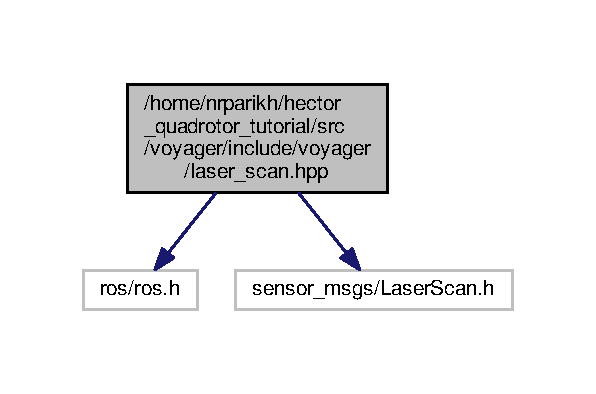
\includegraphics[width=286pt]{laser__scan_8hpp__incl}
\end{center}
\end{figure}
This graph shows which files directly or indirectly include this file\+:
\nopagebreak
\begin{figure}[H]
\begin{center}
\leavevmode
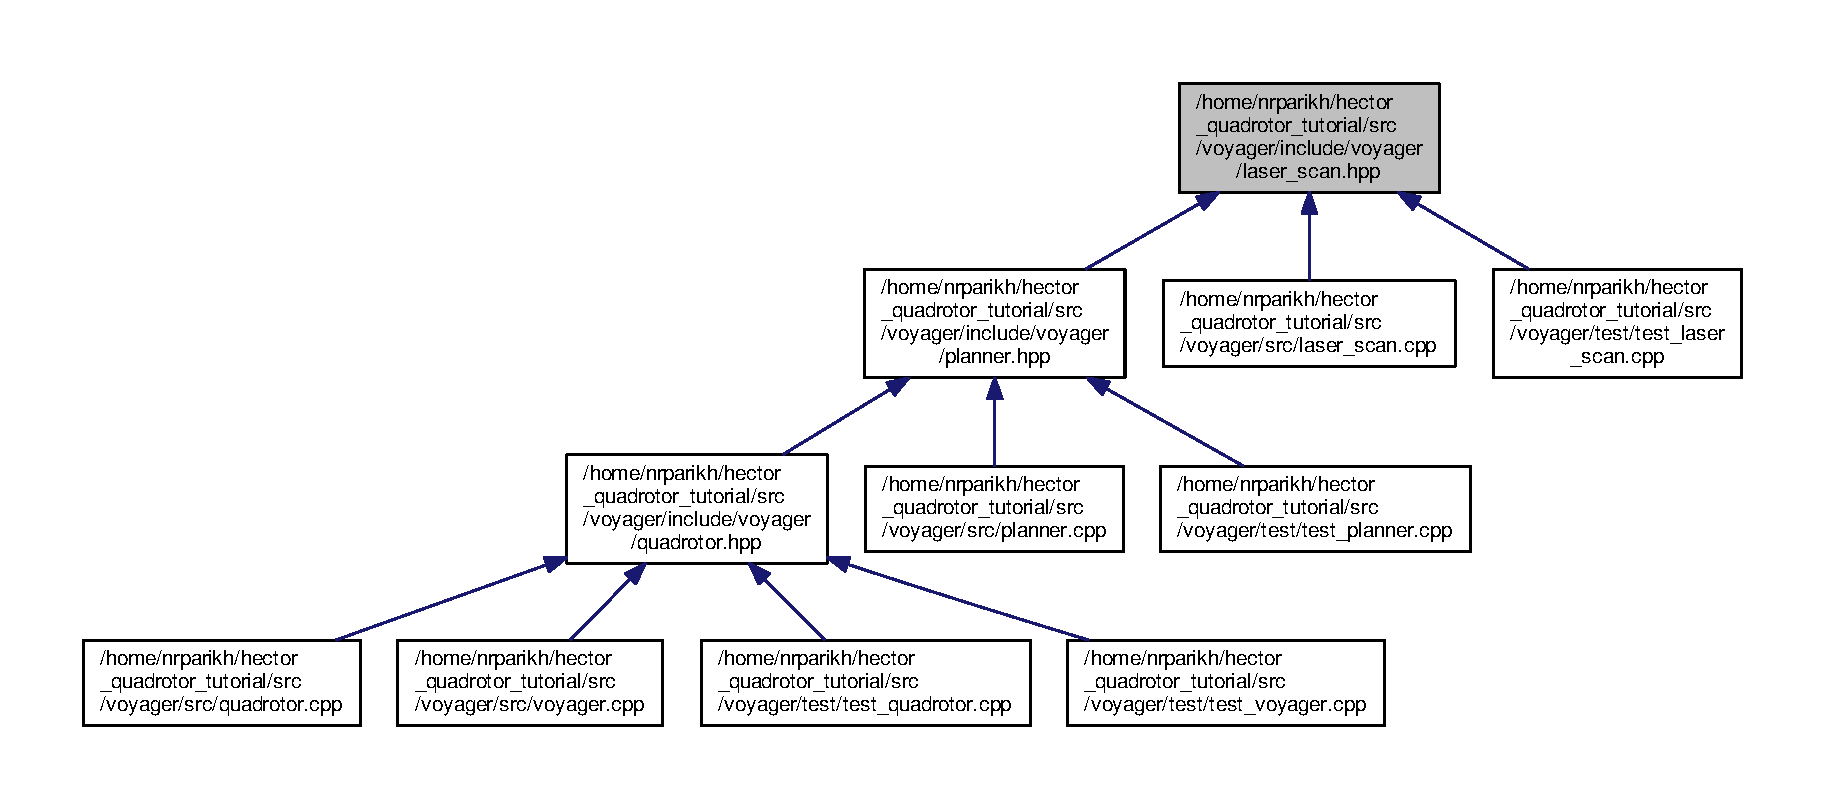
\includegraphics[width=350pt]{laser__scan_8hpp__dep__incl}
\end{center}
\end{figure}
\subsection*{Classes}
\begin{DoxyCompactItemize}
\item 
class \hyperlink{class_laser_scan}{Laser\+Scan}
\end{DoxyCompactItemize}


\subsection{Detailed Description}
D\+E\+S\+C\+R\+I\+P\+T\+I\+ON Header file for the class \hyperlink{class_laser_scan}{Laser\+Scan}. 

\begin{DoxyAuthor}{Author}
nr-\/parikh 
\end{DoxyAuthor}
\begin{DoxyCopyright}{Copyright}
M\+IT license (c) 2017 Neel Parikh 
\end{DoxyCopyright}

\hypertarget{planner_8hpp}{}\section{/home/nrparikh/hector\+\_\+quadrotor\+\_\+tutorial/src/voyager/include/voyager/planner.hpp File Reference}
\label{planner_8hpp}\index{/home/nrparikh/hector\+\_\+quadrotor\+\_\+tutorial/src/voyager/include/voyager/planner.\+hpp@{/home/nrparikh/hector\+\_\+quadrotor\+\_\+tutorial/src/voyager/include/voyager/planner.\+hpp}}


D\+E\+S\+C\+R\+I\+P\+T\+I\+ON Header file for the class \hyperlink{class_planner}{Planner}.  


{\ttfamily \#include $<$geometry\+\_\+msgs/\+Twist.\+h$>$}\\*
{\ttfamily \#include $<$ros/ros.\+h$>$}\\*
{\ttfamily \#include \char`\"{}voyager/laser\+\_\+scan.\+hpp\char`\"{}}\\*
Include dependency graph for planner.\+hpp\+:
\nopagebreak
\begin{figure}[H]
\begin{center}
\leavevmode
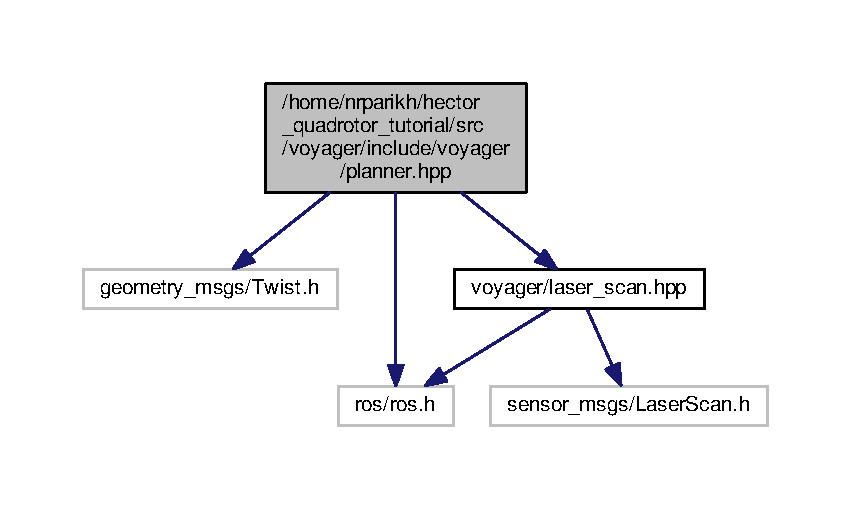
\includegraphics[width=350pt]{planner_8hpp__incl}
\end{center}
\end{figure}
This graph shows which files directly or indirectly include this file\+:
\nopagebreak
\begin{figure}[H]
\begin{center}
\leavevmode
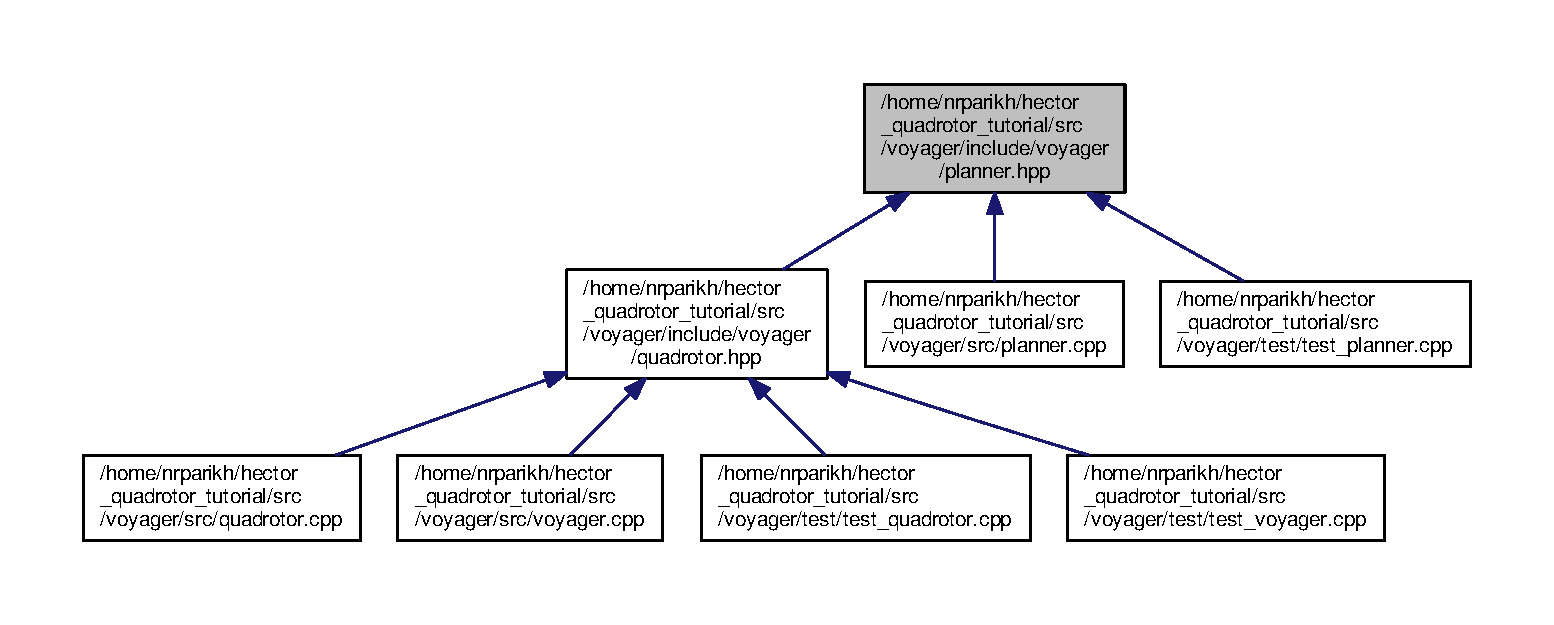
\includegraphics[width=350pt]{planner_8hpp__dep__incl}
\end{center}
\end{figure}
\subsection*{Classes}
\begin{DoxyCompactItemize}
\item 
class \hyperlink{class_planner}{Planner}
\end{DoxyCompactItemize}


\subsection{Detailed Description}
D\+E\+S\+C\+R\+I\+P\+T\+I\+ON Header file for the class \hyperlink{class_planner}{Planner}. 

\begin{DoxyAuthor}{Author}
nr-\/parikh 
\end{DoxyAuthor}
\begin{DoxyCopyright}{Copyright}
M\+IT license (c) 2017 Neel Parikh 
\end{DoxyCopyright}

\hypertarget{quadrotor_8hpp}{}\section{/home/nrparikh/hector\+\_\+quadrotor\+\_\+tutorial/src/voyager/include/voyager/quadrotor.hpp File Reference}
\label{quadrotor_8hpp}\index{/home/nrparikh/hector\+\_\+quadrotor\+\_\+tutorial/src/voyager/include/voyager/quadrotor.\+hpp@{/home/nrparikh/hector\+\_\+quadrotor\+\_\+tutorial/src/voyager/include/voyager/quadrotor.\+hpp}}


D\+E\+S\+C\+R\+I\+P\+T\+I\+ON Header file for the classs \hyperlink{class_quadrotor}{Quadrotor}.  


{\ttfamily \#include $<$geometry\+\_\+msgs/\+Twist.\+h$>$}\\*
{\ttfamily \#include $<$ros/ros.\+h$>$}\\*
{\ttfamily \#include $<$sensor\+\_\+msgs/\+Range.\+h$>$}\\*
{\ttfamily \#include \char`\"{}voyager/explore.\+h\char`\"{}}\\*
{\ttfamily \#include \char`\"{}voyager/planner.\+hpp\char`\"{}}\\*
Include dependency graph for quadrotor.\+hpp\+:
\nopagebreak
\begin{figure}[H]
\begin{center}
\leavevmode
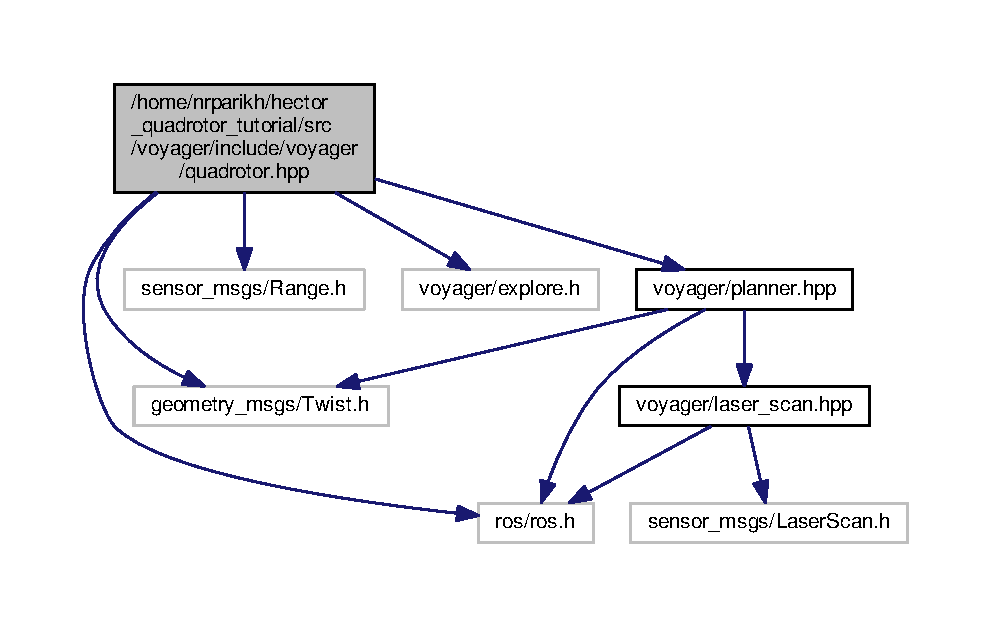
\includegraphics[width=350pt]{quadrotor_8hpp__incl}
\end{center}
\end{figure}
This graph shows which files directly or indirectly include this file\+:
\nopagebreak
\begin{figure}[H]
\begin{center}
\leavevmode
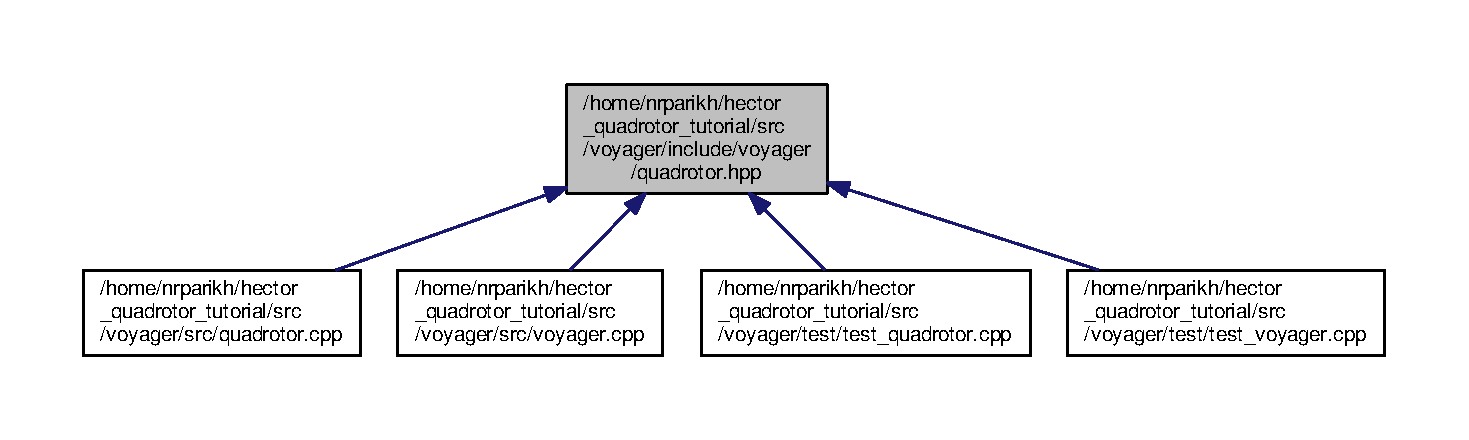
\includegraphics[width=350pt]{quadrotor_8hpp__dep__incl}
\end{center}
\end{figure}
\subsection*{Classes}
\begin{DoxyCompactItemize}
\item 
class \hyperlink{class_quadrotor}{Quadrotor}
\end{DoxyCompactItemize}


\subsection{Detailed Description}
D\+E\+S\+C\+R\+I\+P\+T\+I\+ON Header file for the classs \hyperlink{class_quadrotor}{Quadrotor}. 

\begin{DoxyAuthor}{Author}
nr-\/parikh 
\end{DoxyAuthor}
\begin{DoxyCopyright}{Copyright}
M\+IT license (c) 2017 Neel Parikh 
\end{DoxyCopyright}

\hypertarget{_r_e_a_d_m_e_8md}{}\section{/home/nrparikh/hector\+\_\+quadrotor\+\_\+tutorial/src/voyager/\+R\+E\+A\+D\+ME.md File Reference}
\label{_r_e_a_d_m_e_8md}\index{/home/nrparikh/hector\+\_\+quadrotor\+\_\+tutorial/src/voyager/\+R\+E\+A\+D\+M\+E.\+md@{/home/nrparikh/hector\+\_\+quadrotor\+\_\+tutorial/src/voyager/\+R\+E\+A\+D\+M\+E.\+md}}

\hypertarget{laser__scan_8cpp}{}\section{/home/nrparikh/hector\+\_\+quadrotor\+\_\+tutorial/src/voyager/src/laser\+\_\+scan.cpp File Reference}
\label{laser__scan_8cpp}\index{/home/nrparikh/hector\+\_\+quadrotor\+\_\+tutorial/src/voyager/src/laser\+\_\+scan.\+cpp@{/home/nrparikh/hector\+\_\+quadrotor\+\_\+tutorial/src/voyager/src/laser\+\_\+scan.\+cpp}}


D\+E\+S\+C\+R\+I\+P\+T\+I\+ON Class implementation for the class \hyperlink{class_laser_scan}{Laser\+Scan}.  


{\ttfamily \#include \char`\"{}voyager/laser\+\_\+scan.\+hpp\char`\"{}}\\*
{\ttfamily \#include $<$vector$>$}\\*
Include dependency graph for laser\+\_\+scan.\+cpp\+:
\nopagebreak
\begin{figure}[H]
\begin{center}
\leavevmode
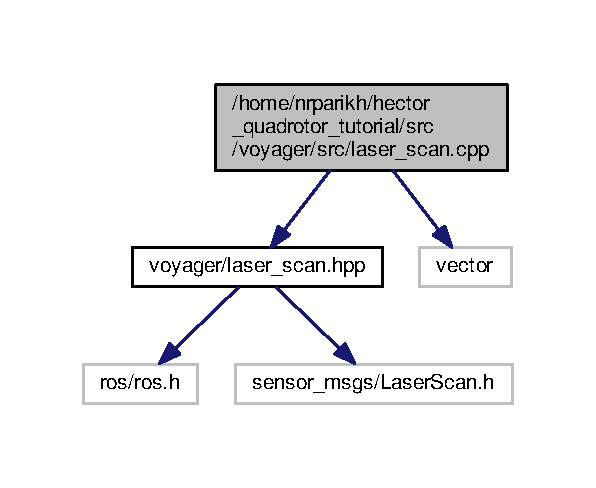
\includegraphics[width=286pt]{laser__scan_8cpp__incl}
\end{center}
\end{figure}


\subsection{Detailed Description}
D\+E\+S\+C\+R\+I\+P\+T\+I\+ON Class implementation for the class \hyperlink{class_laser_scan}{Laser\+Scan}. 

\begin{DoxyAuthor}{Author}
nr-\/parikh 
\end{DoxyAuthor}
\begin{DoxyCopyright}{Copyright}
M\+IT license (c) 2017 Neel Parikh 
\end{DoxyCopyright}

\hypertarget{planner_8cpp}{}\section{/home/nrparikh/hector\+\_\+quadrotor\+\_\+tutorial/src/voyager/src/planner.cpp File Reference}
\label{planner_8cpp}\index{/home/nrparikh/hector\+\_\+quadrotor\+\_\+tutorial/src/voyager/src/planner.\+cpp@{/home/nrparikh/hector\+\_\+quadrotor\+\_\+tutorial/src/voyager/src/planner.\+cpp}}


D\+E\+S\+C\+R\+I\+P\+T\+I\+ON Implementation of the class \hyperlink{class_planner}{Planner}.  


{\ttfamily \#include \char`\"{}voyager/planner.\+hpp\char`\"{}}\\*
{\ttfamily \#include $<$stdlib.\+h$>$}\\*
Include dependency graph for planner.\+cpp\+:
\nopagebreak
\begin{figure}[H]
\begin{center}
\leavevmode
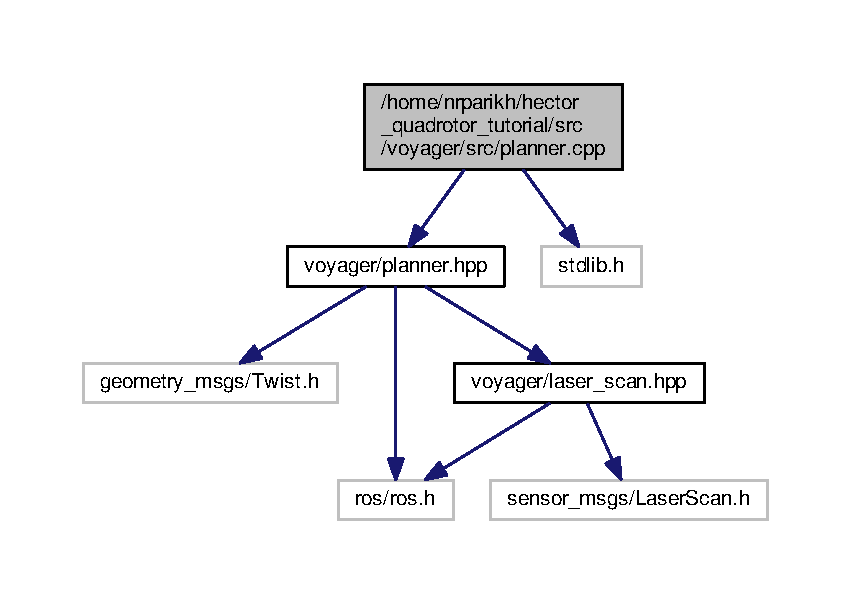
\includegraphics[width=350pt]{planner_8cpp__incl}
\end{center}
\end{figure}


\subsection{Detailed Description}
D\+E\+S\+C\+R\+I\+P\+T\+I\+ON Implementation of the class \hyperlink{class_planner}{Planner}. 

\begin{DoxyAuthor}{Author}
nr-\/parikh 
\end{DoxyAuthor}
\begin{DoxyCopyright}{Copyright}
M\+IT license (c) 2017 Neel Parikh 
\end{DoxyCopyright}

\hypertarget{quadrotor_8cpp}{}\section{/home/nrparikh/hector\+\_\+quadrotor\+\_\+tutorial/src/voyager/src/quadrotor.cpp File Reference}
\label{quadrotor_8cpp}\index{/home/nrparikh/hector\+\_\+quadrotor\+\_\+tutorial/src/voyager/src/quadrotor.\+cpp@{/home/nrparikh/hector\+\_\+quadrotor\+\_\+tutorial/src/voyager/src/quadrotor.\+cpp}}


D\+E\+S\+C\+R\+I\+P\+T\+I\+ON Implementation of the class \hyperlink{class_quadrotor}{Quadrotor}.  


{\ttfamily \#include \char`\"{}voyager/quadrotor.\+hpp\char`\"{}}\\*
{\ttfamily \#include $<$cmath$>$}\\*
Include dependency graph for quadrotor.\+cpp\+:
\nopagebreak
\begin{figure}[H]
\begin{center}
\leavevmode
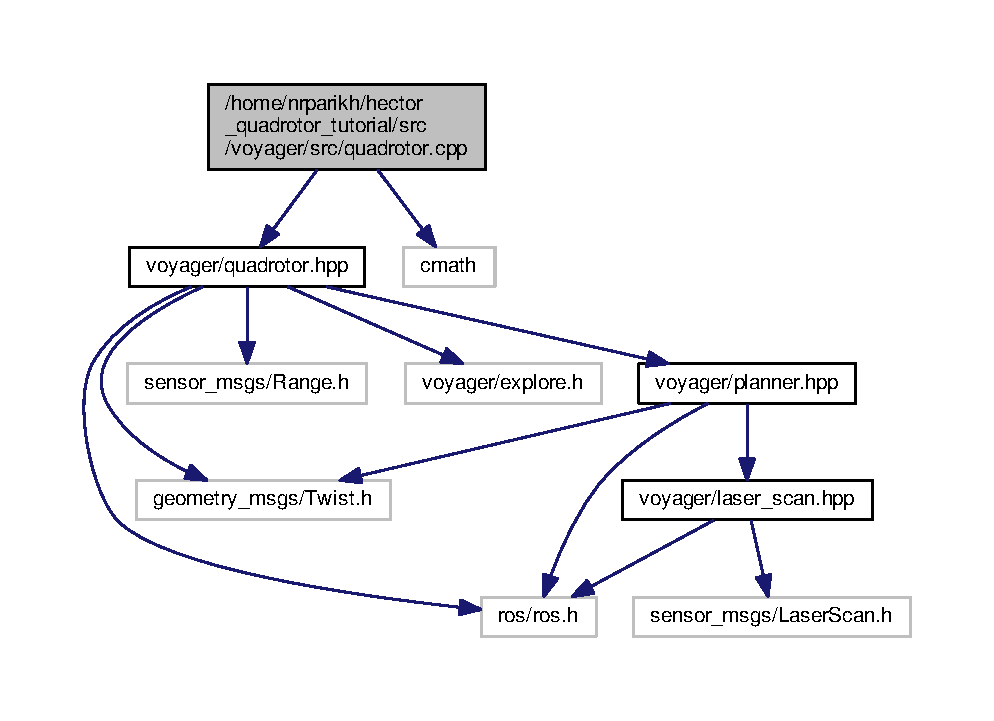
\includegraphics[width=350pt]{quadrotor_8cpp__incl}
\end{center}
\end{figure}


\subsection{Detailed Description}
D\+E\+S\+C\+R\+I\+P\+T\+I\+ON Implementation of the class \hyperlink{class_quadrotor}{Quadrotor}. 

\begin{DoxyAuthor}{Author}
nr-\/parikh 
\end{DoxyAuthor}
\begin{DoxyCopyright}{Copyright}
M\+IT license (c) 2017 Neel Parikh 
\end{DoxyCopyright}

\hypertarget{voyager_8cpp}{}\section{/home/nrparikh/hector\+\_\+quadrotor\+\_\+tutorial/src/voyager/src/voyager.cpp File Reference}
\label{voyager_8cpp}\index{/home/nrparikh/hector\+\_\+quadrotor\+\_\+tutorial/src/voyager/src/voyager.\+cpp@{/home/nrparikh/hector\+\_\+quadrotor\+\_\+tutorial/src/voyager/src/voyager.\+cpp}}


D\+E\+S\+C\+R\+I\+P\+T\+I\+ON Main file for the package voyager.  


{\ttfamily \#include $<$hector\+\_\+uav\+\_\+msgs/\+Enable\+Motors.\+h$>$}\\*
{\ttfamily \#include $<$ros/ros.\+h$>$}\\*
{\ttfamily \#include $<$std\+\_\+msgs/\+String.\+h$>$}\\*
{\ttfamily \#include \char`\"{}voyager/explore.\+h\char`\"{}}\\*
{\ttfamily \#include \char`\"{}voyager/quadrotor.\+hpp\char`\"{}}\\*
Include dependency graph for voyager.\+cpp\+:
\nopagebreak
\begin{figure}[H]
\begin{center}
\leavevmode
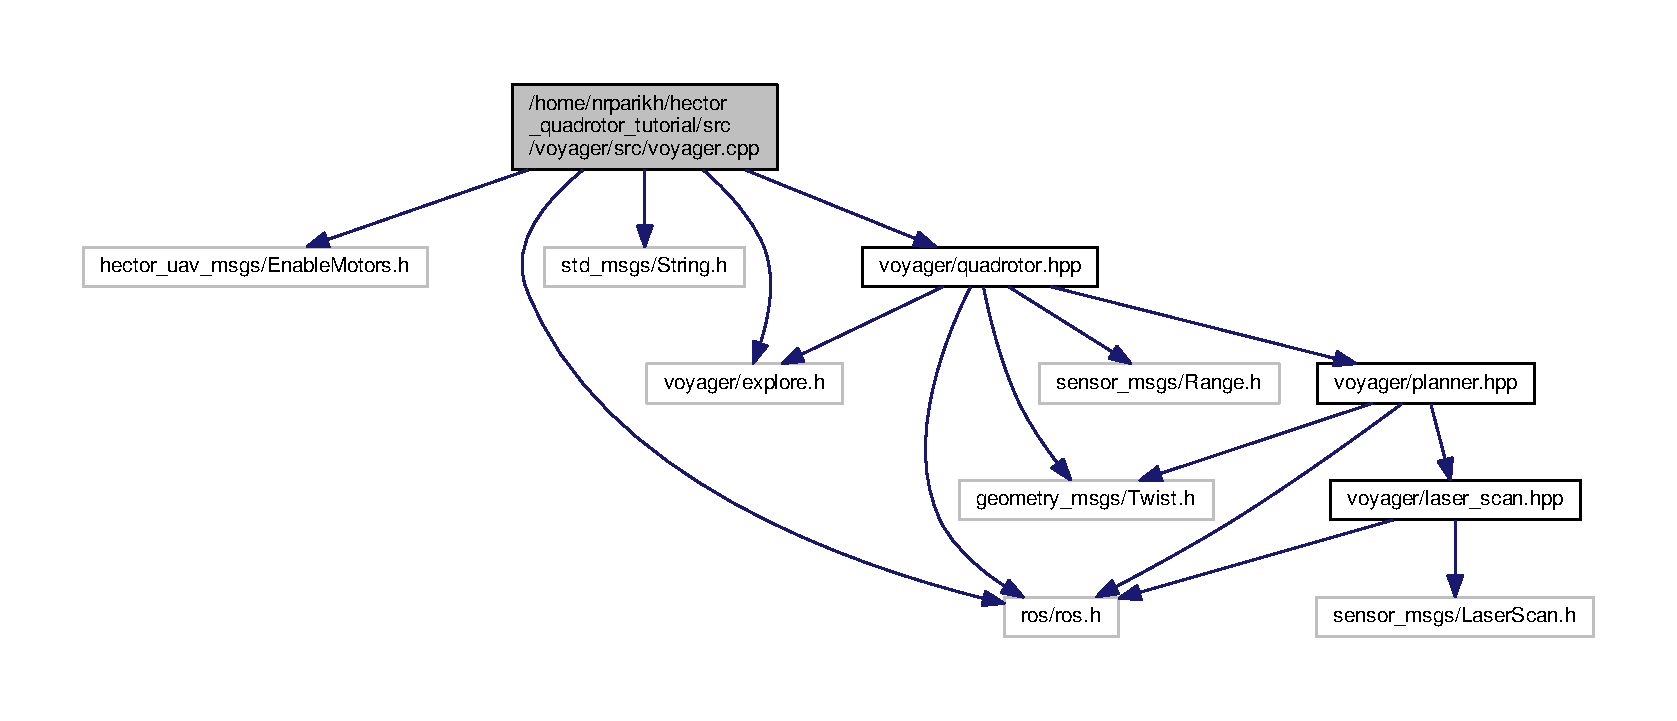
\includegraphics[width=350pt]{voyager_8cpp__incl}
\end{center}
\end{figure}
\subsection*{Functions}
\begin{DoxyCompactItemize}
\item 
int \hyperlink{voyager_8cpp_a3c04138a5bfe5d72780bb7e82a18e627}{main} (int argc, char $\ast$$\ast$argv)
\end{DoxyCompactItemize}


\subsection{Detailed Description}
D\+E\+S\+C\+R\+I\+P\+T\+I\+ON Main file for the package voyager. 

\begin{DoxyAuthor}{Author}
nr-\/parikh 
\end{DoxyAuthor}
\begin{DoxyCopyright}{Copyright}
M\+IT license (c) 2017 Neel Parikh 
\end{DoxyCopyright}


\subsection{Function Documentation}
\index{voyager.\+cpp@{voyager.\+cpp}!main@{main}}
\index{main@{main}!voyager.\+cpp@{voyager.\+cpp}}
\subsubsection[{\texorpdfstring{main(int argc, char $\ast$$\ast$argv)}{main(int argc, char **argv)}}]{\setlength{\rightskip}{0pt plus 5cm}int main (
\begin{DoxyParamCaption}
\item[{int}]{argc, }
\item[{char $\ast$$\ast$}]{argv}
\end{DoxyParamCaption}
)}\hypertarget{voyager_8cpp_a3c04138a5bfe5d72780bb7e82a18e627}{}\label{voyager_8cpp_a3c04138a5bfe5d72780bb7e82a18e627}


Definition at line 40 of file voyager.\+cpp.


\hypertarget{test__laser__scan_8cpp}{}\section{/home/nrparikh/hector\+\_\+quadrotor\+\_\+tutorial/src/voyager/test/test\+\_\+laser\+\_\+scan.cpp File Reference}
\label{test__laser__scan_8cpp}\index{/home/nrparikh/hector\+\_\+quadrotor\+\_\+tutorial/src/voyager/test/test\+\_\+laser\+\_\+scan.\+cpp@{/home/nrparikh/hector\+\_\+quadrotor\+\_\+tutorial/src/voyager/test/test\+\_\+laser\+\_\+scan.\+cpp}}


D\+E\+S\+C\+R\+I\+P\+T\+I\+ON Unit tests for the class \hyperlink{class_laser_scan}{Laser\+Scan}.  


{\ttfamily \#include $<$gtest/gtest.\+h$>$}\\*
{\ttfamily \#include $<$ros/ros.\+h$>$}\\*
{\ttfamily \#include \char`\"{}voyager/laser\+\_\+scan.\+hpp\char`\"{}}\\*
Include dependency graph for test\+\_\+laser\+\_\+scan.\+cpp\+:
\nopagebreak
\begin{figure}[H]
\begin{center}
\leavevmode
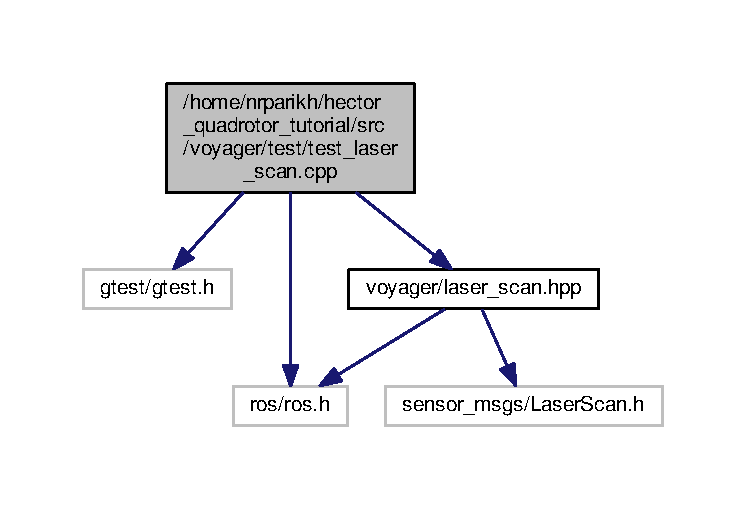
\includegraphics[width=350pt]{test__laser__scan_8cpp__incl}
\end{center}
\end{figure}
\subsection*{Functions}
\begin{DoxyCompactItemize}
\item 
\hyperlink{test__laser__scan_8cpp_ab63e43e61ab0a01057979ceeb03998fe}{T\+E\+ST} (T\+E\+S\+T\+\_\+\+L\+A\+S\+E\+R\+S\+C\+AN, Test\+Laser\+Scan\+Running)
\item 
\hyperlink{test__laser__scan_8cpp_a778002901bca09a9418afb01933fdebf}{T\+E\+ST} (T\+E\+S\+T\+\_\+\+L\+A\+S\+E\+R\+S\+C\+AN, Test\+Laser\+Scan\+Subscriber)
\item 
\hyperlink{test__laser__scan_8cpp_aa6a155de03aaee6c79d4ccb5cb7b22fb}{T\+E\+ST} (T\+E\+S\+T\+\_\+\+L\+A\+S\+E\+R\+S\+C\+AN, Test\+Laser\+Scan\+Check\+Collision)
\end{DoxyCompactItemize}


\subsection{Detailed Description}
D\+E\+S\+C\+R\+I\+P\+T\+I\+ON Unit tests for the class \hyperlink{class_laser_scan}{Laser\+Scan}. 

\begin{DoxyAuthor}{Author}
nr-\/parikh 
\end{DoxyAuthor}
\begin{DoxyCopyright}{Copyright}
M\+IT license (c) 2017 Neel Parikh 
\end{DoxyCopyright}


\subsection{Function Documentation}
\index{test\+\_\+laser\+\_\+scan.\+cpp@{test\+\_\+laser\+\_\+scan.\+cpp}!T\+E\+ST@{T\+E\+ST}}
\index{T\+E\+ST@{T\+E\+ST}!test\+\_\+laser\+\_\+scan.\+cpp@{test\+\_\+laser\+\_\+scan.\+cpp}}
\subsubsection[{\texorpdfstring{T\+E\+S\+T(\+T\+E\+S\+T\+\_\+\+L\+A\+S\+E\+R\+S\+C\+A\+N, Test\+Laser\+Scan\+Running)}{TEST(TEST_LASERSCAN, TestLaserScanRunning)}}]{\setlength{\rightskip}{0pt plus 5cm}T\+E\+ST (
\begin{DoxyParamCaption}
\item[{T\+E\+S\+T\+\_\+\+L\+A\+S\+E\+R\+S\+C\+AN}]{, }
\item[{Test\+Laser\+Scan\+Running}]{}
\end{DoxyParamCaption}
)}\hypertarget{test__laser__scan_8cpp_ab63e43e61ab0a01057979ceeb03998fe}{}\label{test__laser__scan_8cpp_ab63e43e61ab0a01057979ceeb03998fe}


Definition at line 38 of file test\+\_\+laser\+\_\+scan.\+cpp.

\index{test\+\_\+laser\+\_\+scan.\+cpp@{test\+\_\+laser\+\_\+scan.\+cpp}!T\+E\+ST@{T\+E\+ST}}
\index{T\+E\+ST@{T\+E\+ST}!test\+\_\+laser\+\_\+scan.\+cpp@{test\+\_\+laser\+\_\+scan.\+cpp}}
\subsubsection[{\texorpdfstring{T\+E\+S\+T(\+T\+E\+S\+T\+\_\+\+L\+A\+S\+E\+R\+S\+C\+A\+N, Test\+Laser\+Scan\+Subscriber)}{TEST(TEST_LASERSCAN, TestLaserScanSubscriber)}}]{\setlength{\rightskip}{0pt plus 5cm}T\+E\+ST (
\begin{DoxyParamCaption}
\item[{T\+E\+S\+T\+\_\+\+L\+A\+S\+E\+R\+S\+C\+AN}]{, }
\item[{Test\+Laser\+Scan\+Subscriber}]{}
\end{DoxyParamCaption}
)}\hypertarget{test__laser__scan_8cpp_a778002901bca09a9418afb01933fdebf}{}\label{test__laser__scan_8cpp_a778002901bca09a9418afb01933fdebf}


Definition at line 45 of file test\+\_\+laser\+\_\+scan.\+cpp.

\index{test\+\_\+laser\+\_\+scan.\+cpp@{test\+\_\+laser\+\_\+scan.\+cpp}!T\+E\+ST@{T\+E\+ST}}
\index{T\+E\+ST@{T\+E\+ST}!test\+\_\+laser\+\_\+scan.\+cpp@{test\+\_\+laser\+\_\+scan.\+cpp}}
\subsubsection[{\texorpdfstring{T\+E\+S\+T(\+T\+E\+S\+T\+\_\+\+L\+A\+S\+E\+R\+S\+C\+A\+N, Test\+Laser\+Scan\+Check\+Collision)}{TEST(TEST_LASERSCAN, TestLaserScanCheckCollision)}}]{\setlength{\rightskip}{0pt plus 5cm}T\+E\+ST (
\begin{DoxyParamCaption}
\item[{T\+E\+S\+T\+\_\+\+L\+A\+S\+E\+R\+S\+C\+AN}]{, }
\item[{Test\+Laser\+Scan\+Check\+Collision}]{}
\end{DoxyParamCaption}
)}\hypertarget{test__laser__scan_8cpp_aa6a155de03aaee6c79d4ccb5cb7b22fb}{}\label{test__laser__scan_8cpp_aa6a155de03aaee6c79d4ccb5cb7b22fb}


Definition at line 56 of file test\+\_\+laser\+\_\+scan.\+cpp.


\hypertarget{test__planner_8cpp}{}\section{/home/nrparikh/hector\+\_\+quadrotor\+\_\+tutorial/src/voyager/test/test\+\_\+planner.cpp File Reference}
\label{test__planner_8cpp}\index{/home/nrparikh/hector\+\_\+quadrotor\+\_\+tutorial/src/voyager/test/test\+\_\+planner.\+cpp@{/home/nrparikh/hector\+\_\+quadrotor\+\_\+tutorial/src/voyager/test/test\+\_\+planner.\+cpp}}


D\+E\+S\+C\+R\+I\+P\+T\+I\+ON Unit tests for the class \hyperlink{class_planner}{Planner}.  


{\ttfamily \#include $<$gtest/gtest.\+h$>$}\\*
{\ttfamily \#include $<$ros/ros.\+h$>$}\\*
{\ttfamily \#include \char`\"{}voyager/planner.\+hpp\char`\"{}}\\*
Include dependency graph for test\+\_\+planner.\+cpp\+:
\nopagebreak
\begin{figure}[H]
\begin{center}
\leavevmode
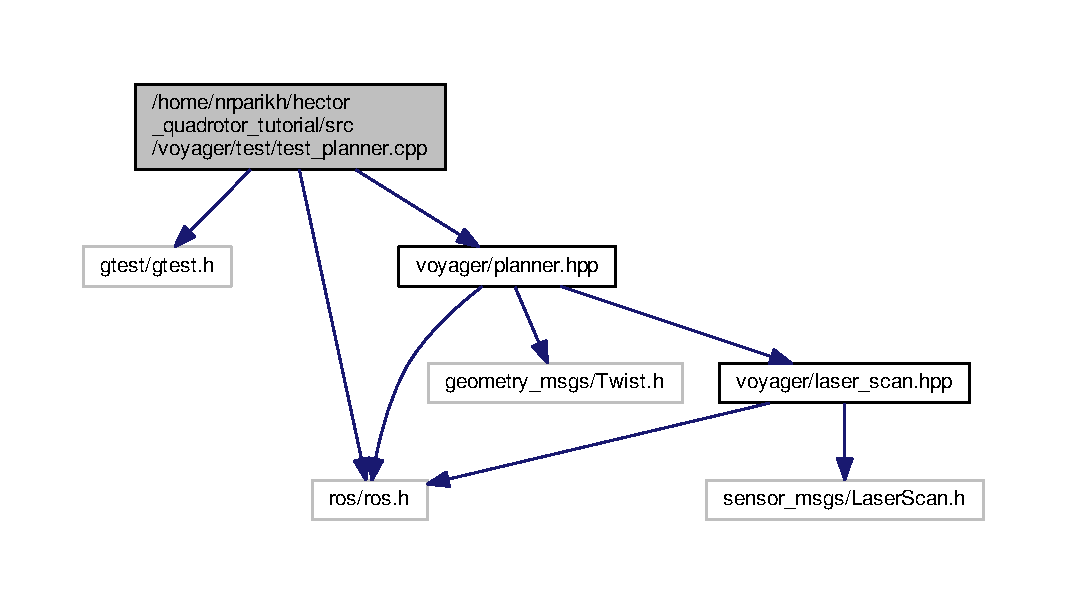
\includegraphics[width=350pt]{test__planner_8cpp__incl}
\end{center}
\end{figure}
\subsection*{Functions}
\begin{DoxyCompactItemize}
\item 
void \hyperlink{test__planner_8cpp_a4e8590bd2ff13dc5b642d8577241b4bd}{call\+Back} (const geometry\+\_\+msgs\+::\+Twist \&msg)
\item 
\hyperlink{test__planner_8cpp_a6cc633c0c1e6eb62dcb2d6401fe06228}{T\+E\+ST} (T\+E\+S\+T\+\_\+\+P\+L\+A\+N\+N\+ER, Test\+Planner\+Alive)
\item 
\hyperlink{test__planner_8cpp_ae9632ae25f20b06a8660bf1de0e7826f}{T\+E\+ST} (T\+E\+S\+T\+\_\+\+P\+L\+A\+N\+N\+ER, Test\+Planner\+Publisher)
\end{DoxyCompactItemize}


\subsection{Detailed Description}
D\+E\+S\+C\+R\+I\+P\+T\+I\+ON Unit tests for the class \hyperlink{class_planner}{Planner}. 

\begin{DoxyAuthor}{Author}
nr-\/parikh 
\end{DoxyAuthor}
\begin{DoxyCopyright}{Copyright}
M\+IT license (c) 2017 Neel Parikh 
\end{DoxyCopyright}


\subsection{Function Documentation}
\index{test\+\_\+planner.\+cpp@{test\+\_\+planner.\+cpp}!call\+Back@{call\+Back}}
\index{call\+Back@{call\+Back}!test\+\_\+planner.\+cpp@{test\+\_\+planner.\+cpp}}
\subsubsection[{\texorpdfstring{call\+Back(const geometry\+\_\+msgs\+::\+Twist \&msg)}{callBack(const geometry_msgs::Twist &msg)}}]{\setlength{\rightskip}{0pt plus 5cm}void call\+Back (
\begin{DoxyParamCaption}
\item[{const geometry\+\_\+msgs\+::\+Twist \&}]{msg}
\end{DoxyParamCaption}
)}\hypertarget{test__planner_8cpp_a4e8590bd2ff13dc5b642d8577241b4bd}{}\label{test__planner_8cpp_a4e8590bd2ff13dc5b642d8577241b4bd}


Definition at line 38 of file test\+\_\+planner.\+cpp.

\index{test\+\_\+planner.\+cpp@{test\+\_\+planner.\+cpp}!T\+E\+ST@{T\+E\+ST}}
\index{T\+E\+ST@{T\+E\+ST}!test\+\_\+planner.\+cpp@{test\+\_\+planner.\+cpp}}
\subsubsection[{\texorpdfstring{T\+E\+S\+T(\+T\+E\+S\+T\+\_\+\+P\+L\+A\+N\+N\+E\+R, Test\+Planner\+Alive)}{TEST(TEST_PLANNER, TestPlannerAlive)}}]{\setlength{\rightskip}{0pt plus 5cm}T\+E\+ST (
\begin{DoxyParamCaption}
\item[{T\+E\+S\+T\+\_\+\+P\+L\+A\+N\+N\+ER}]{, }
\item[{Test\+Planner\+Alive}]{}
\end{DoxyParamCaption}
)}\hypertarget{test__planner_8cpp_a6cc633c0c1e6eb62dcb2d6401fe06228}{}\label{test__planner_8cpp_a6cc633c0c1e6eb62dcb2d6401fe06228}


Definition at line 42 of file test\+\_\+planner.\+cpp.

\index{test\+\_\+planner.\+cpp@{test\+\_\+planner.\+cpp}!T\+E\+ST@{T\+E\+ST}}
\index{T\+E\+ST@{T\+E\+ST}!test\+\_\+planner.\+cpp@{test\+\_\+planner.\+cpp}}
\subsubsection[{\texorpdfstring{T\+E\+S\+T(\+T\+E\+S\+T\+\_\+\+P\+L\+A\+N\+N\+E\+R, Test\+Planner\+Publisher)}{TEST(TEST_PLANNER, TestPlannerPublisher)}}]{\setlength{\rightskip}{0pt plus 5cm}T\+E\+ST (
\begin{DoxyParamCaption}
\item[{T\+E\+S\+T\+\_\+\+P\+L\+A\+N\+N\+ER}]{, }
\item[{Test\+Planner\+Publisher}]{}
\end{DoxyParamCaption}
)}\hypertarget{test__planner_8cpp_ae9632ae25f20b06a8660bf1de0e7826f}{}\label{test__planner_8cpp_ae9632ae25f20b06a8660bf1de0e7826f}


Definition at line 49 of file test\+\_\+planner.\+cpp.


\hypertarget{test__quadrotor_8cpp}{}\section{/home/nrparikh/hector\+\_\+quadrotor\+\_\+tutorial/src/voyager/test/test\+\_\+quadrotor.cpp File Reference}
\label{test__quadrotor_8cpp}\index{/home/nrparikh/hector\+\_\+quadrotor\+\_\+tutorial/src/voyager/test/test\+\_\+quadrotor.\+cpp@{/home/nrparikh/hector\+\_\+quadrotor\+\_\+tutorial/src/voyager/test/test\+\_\+quadrotor.\+cpp}}
{\ttfamily \#include $<$gtest/gtest.\+h$>$}\\*
{\ttfamily \#include $<$ros/ros.\+h$>$}\\*
{\ttfamily \#include \char`\"{}voyager/quadrotor.\+hpp\char`\"{}}\\*
Include dependency graph for test\+\_\+quadrotor.\+cpp\+:
\nopagebreak
\begin{figure}[H]
\begin{center}
\leavevmode
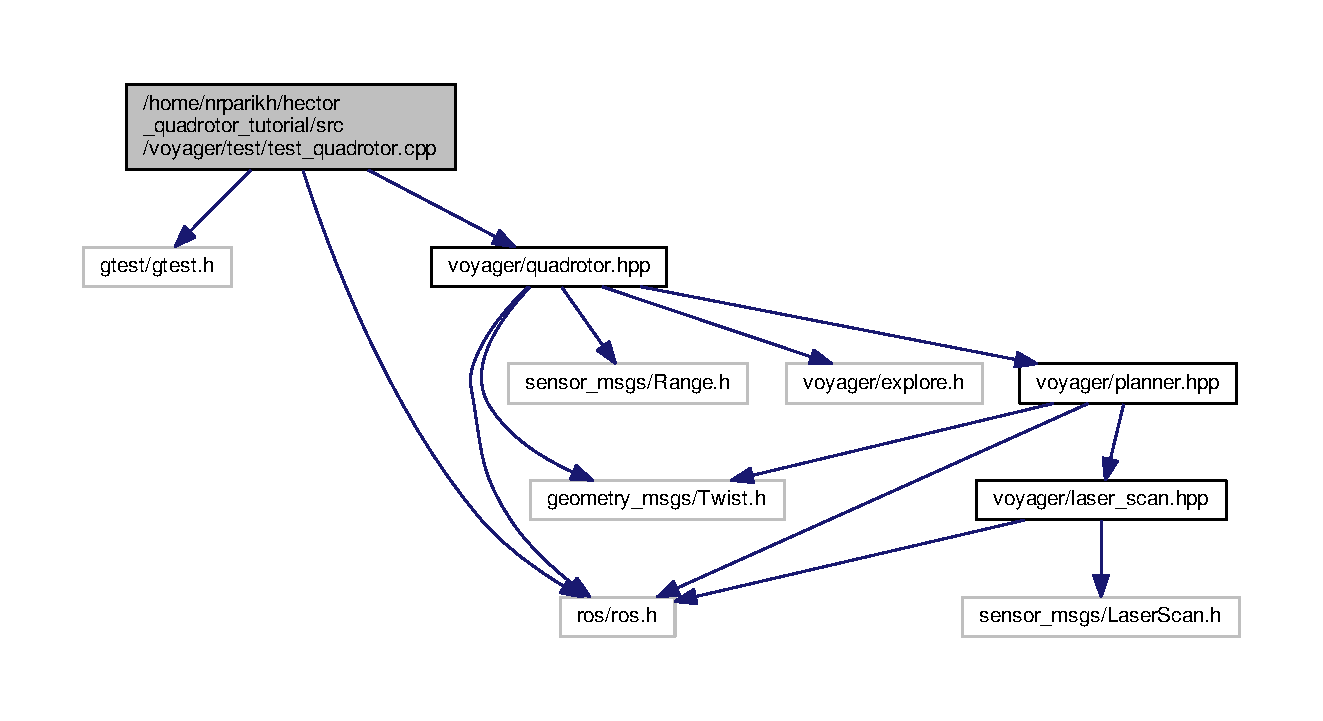
\includegraphics[width=350pt]{test__quadrotor_8cpp__incl}
\end{center}
\end{figure}
\subsection*{Functions}
\begin{DoxyCompactItemize}
\item 
\hyperlink{test__quadrotor_8cpp_aff119c40d6a4e80d38350d4c9c66b739}{T\+E\+ST} (T\+E\+S\+T\+\_\+\+Q\+U\+A\+D\+R\+O\+T\+OR, Test\+Quadrotor\+Running)
\item 
\hyperlink{test__quadrotor_8cpp_a5da2c4a68312f5290c17e99315898ea1}{T\+E\+ST} (T\+E\+S\+T\+\_\+\+Q\+U\+A\+D\+R\+O\+T\+OR, Test\+Quadrotor\+Height\+Subscriber)
\item 
\hyperlink{test__quadrotor_8cpp_adb6f8a6a62df25a7252d0255f56ccb49}{T\+E\+ST} (T\+E\+S\+T\+\_\+\+Q\+U\+A\+D\+R\+O\+T\+OR, Test\+Quadrotor\+Get\+Height)
\end{DoxyCompactItemize}


\subsection{Function Documentation}
\index{test\+\_\+quadrotor.\+cpp@{test\+\_\+quadrotor.\+cpp}!T\+E\+ST@{T\+E\+ST}}
\index{T\+E\+ST@{T\+E\+ST}!test\+\_\+quadrotor.\+cpp@{test\+\_\+quadrotor.\+cpp}}
\subsubsection[{\texorpdfstring{T\+E\+S\+T(\+T\+E\+S\+T\+\_\+\+Q\+U\+A\+D\+R\+O\+T\+O\+R, Test\+Quadrotor\+Running)}{TEST(TEST_QUADROTOR, TestQuadrotorRunning)}}]{\setlength{\rightskip}{0pt plus 5cm}T\+E\+ST (
\begin{DoxyParamCaption}
\item[{T\+E\+S\+T\+\_\+\+Q\+U\+A\+D\+R\+O\+T\+OR}]{, }
\item[{Test\+Quadrotor\+Running}]{}
\end{DoxyParamCaption}
)}\hypertarget{test__quadrotor_8cpp_aff119c40d6a4e80d38350d4c9c66b739}{}\label{test__quadrotor_8cpp_aff119c40d6a4e80d38350d4c9c66b739}


Definition at line 38 of file test\+\_\+quadrotor.\+cpp.

\index{test\+\_\+quadrotor.\+cpp@{test\+\_\+quadrotor.\+cpp}!T\+E\+ST@{T\+E\+ST}}
\index{T\+E\+ST@{T\+E\+ST}!test\+\_\+quadrotor.\+cpp@{test\+\_\+quadrotor.\+cpp}}
\subsubsection[{\texorpdfstring{T\+E\+S\+T(\+T\+E\+S\+T\+\_\+\+Q\+U\+A\+D\+R\+O\+T\+O\+R, Test\+Quadrotor\+Height\+Subscriber)}{TEST(TEST_QUADROTOR, TestQuadrotorHeightSubscriber)}}]{\setlength{\rightskip}{0pt plus 5cm}T\+E\+ST (
\begin{DoxyParamCaption}
\item[{T\+E\+S\+T\+\_\+\+Q\+U\+A\+D\+R\+O\+T\+OR}]{, }
\item[{Test\+Quadrotor\+Height\+Subscriber}]{}
\end{DoxyParamCaption}
)}\hypertarget{test__quadrotor_8cpp_a5da2c4a68312f5290c17e99315898ea1}{}\label{test__quadrotor_8cpp_a5da2c4a68312f5290c17e99315898ea1}


Definition at line 45 of file test\+\_\+quadrotor.\+cpp.

\index{test\+\_\+quadrotor.\+cpp@{test\+\_\+quadrotor.\+cpp}!T\+E\+ST@{T\+E\+ST}}
\index{T\+E\+ST@{T\+E\+ST}!test\+\_\+quadrotor.\+cpp@{test\+\_\+quadrotor.\+cpp}}
\subsubsection[{\texorpdfstring{T\+E\+S\+T(\+T\+E\+S\+T\+\_\+\+Q\+U\+A\+D\+R\+O\+T\+O\+R, Test\+Quadrotor\+Get\+Height)}{TEST(TEST_QUADROTOR, TestQuadrotorGetHeight)}}]{\setlength{\rightskip}{0pt plus 5cm}T\+E\+ST (
\begin{DoxyParamCaption}
\item[{T\+E\+S\+T\+\_\+\+Q\+U\+A\+D\+R\+O\+T\+OR}]{, }
\item[{Test\+Quadrotor\+Get\+Height}]{}
\end{DoxyParamCaption}
)}\hypertarget{test__quadrotor_8cpp_adb6f8a6a62df25a7252d0255f56ccb49}{}\label{test__quadrotor_8cpp_adb6f8a6a62df25a7252d0255f56ccb49}


Definition at line 58 of file test\+\_\+quadrotor.\+cpp.


\hypertarget{test__voyager_8cpp}{}\section{/home/nrparikh/hector\+\_\+quadrotor\+\_\+tutorial/src/voyager/test/test\+\_\+voyager.cpp File Reference}
\label{test__voyager_8cpp}\index{/home/nrparikh/hector\+\_\+quadrotor\+\_\+tutorial/src/voyager/test/test\+\_\+voyager.\+cpp@{/home/nrparikh/hector\+\_\+quadrotor\+\_\+tutorial/src/voyager/test/test\+\_\+voyager.\+cpp}}


D\+E\+S\+C\+R\+I\+P\+T\+I\+ON Test file for checking the service.  


{\ttfamily \#include $<$gtest/gtest.\+h$>$}\\*
{\ttfamily \#include $<$ros/ros.\+h$>$}\\*
{\ttfamily \#include $<$ros/service\+\_\+client.\+h$>$}\\*
{\ttfamily \#include \char`\"{}voyager/explore.\+h\char`\"{}}\\*
{\ttfamily \#include \char`\"{}voyager/quadrotor.\+hpp\char`\"{}}\\*
Include dependency graph for test\+\_\+voyager.\+cpp\+:
\nopagebreak
\begin{figure}[H]
\begin{center}
\leavevmode
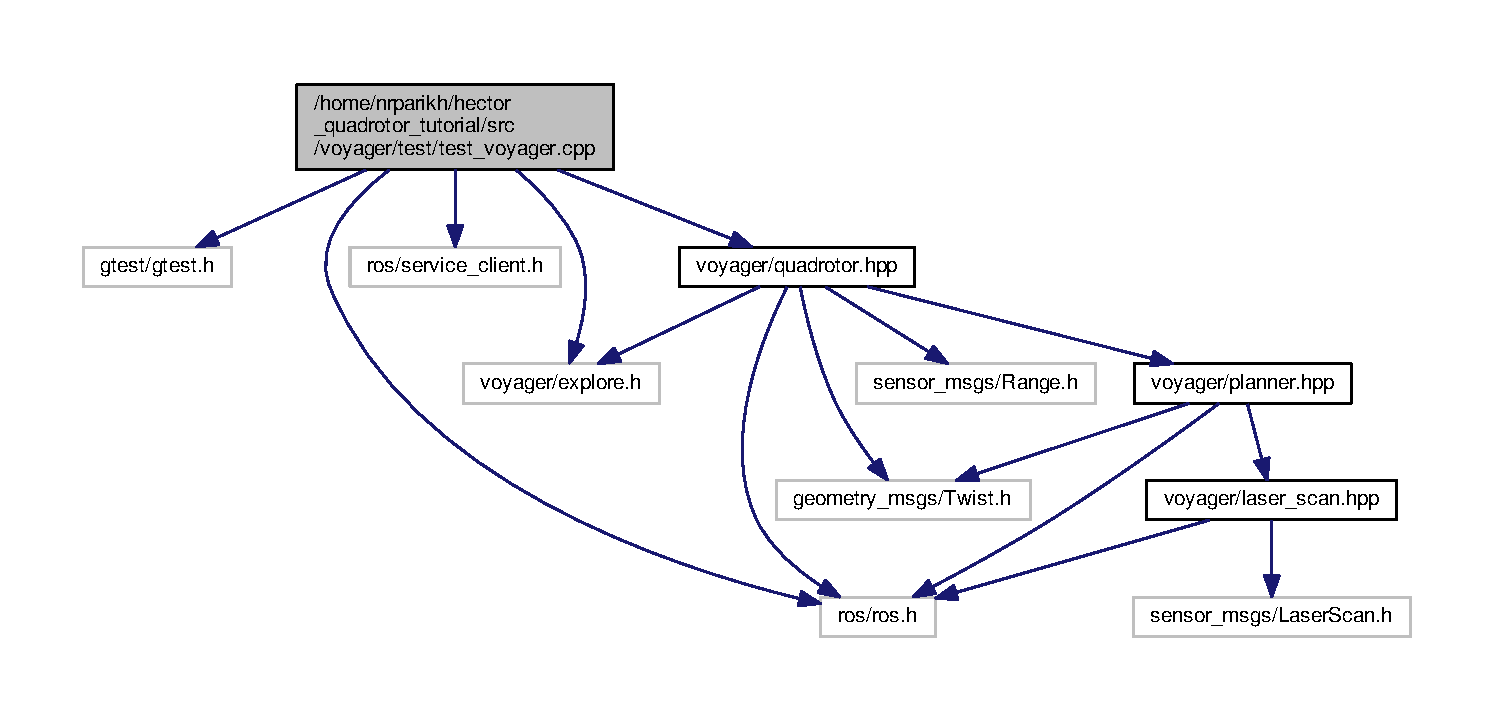
\includegraphics[width=350pt]{test__voyager_8cpp__incl}
\end{center}
\end{figure}
\subsection*{Functions}
\begin{DoxyCompactItemize}
\item 
\hyperlink{test__voyager_8cpp_ad57033bb9599728e014adacff50fe6b7}{T\+E\+ST} (T\+E\+S\+T\+\_\+\+V\+O\+Y\+A\+G\+ER, Test\+Voyager\+Service)
\item 
\hyperlink{test__voyager_8cpp_a84c9631503167ea7cf07737919c9fa81}{T\+E\+ST} (T\+E\+S\+T\+\_\+\+V\+O\+Y\+A\+G\+ER, Test\+Voyager\+Service\+Call)
\end{DoxyCompactItemize}


\subsection{Detailed Description}
D\+E\+S\+C\+R\+I\+P\+T\+I\+ON Test file for checking the service. 

\begin{DoxyAuthor}{Author}
nr-\/parikh 
\end{DoxyAuthor}
\begin{DoxyCopyright}{Copyright}
M\+IT license (c) 2017 Neel Parikh 
\end{DoxyCopyright}


\subsection{Function Documentation}
\index{test\+\_\+voyager.\+cpp@{test\+\_\+voyager.\+cpp}!T\+E\+ST@{T\+E\+ST}}
\index{T\+E\+ST@{T\+E\+ST}!test\+\_\+voyager.\+cpp@{test\+\_\+voyager.\+cpp}}
\subsubsection[{\texorpdfstring{T\+E\+S\+T(\+T\+E\+S\+T\+\_\+\+V\+O\+Y\+A\+G\+E\+R, Test\+Voyager\+Service)}{TEST(TEST_VOYAGER, TestVoyagerService)}}]{\setlength{\rightskip}{0pt plus 5cm}T\+E\+ST (
\begin{DoxyParamCaption}
\item[{T\+E\+S\+T\+\_\+\+V\+O\+Y\+A\+G\+ER}]{, }
\item[{Test\+Voyager\+Service}]{}
\end{DoxyParamCaption}
)}\hypertarget{test__voyager_8cpp_ad57033bb9599728e014adacff50fe6b7}{}\label{test__voyager_8cpp_ad57033bb9599728e014adacff50fe6b7}


Definition at line 40 of file test\+\_\+voyager.\+cpp.

\index{test\+\_\+voyager.\+cpp@{test\+\_\+voyager.\+cpp}!T\+E\+ST@{T\+E\+ST}}
\index{T\+E\+ST@{T\+E\+ST}!test\+\_\+voyager.\+cpp@{test\+\_\+voyager.\+cpp}}
\subsubsection[{\texorpdfstring{T\+E\+S\+T(\+T\+E\+S\+T\+\_\+\+V\+O\+Y\+A\+G\+E\+R, Test\+Voyager\+Service\+Call)}{TEST(TEST_VOYAGER, TestVoyagerServiceCall)}}]{\setlength{\rightskip}{0pt plus 5cm}T\+E\+ST (
\begin{DoxyParamCaption}
\item[{T\+E\+S\+T\+\_\+\+V\+O\+Y\+A\+G\+ER}]{, }
\item[{Test\+Voyager\+Service\+Call}]{}
\end{DoxyParamCaption}
)}\hypertarget{test__voyager_8cpp_a84c9631503167ea7cf07737919c9fa81}{}\label{test__voyager_8cpp_a84c9631503167ea7cf07737919c9fa81}


Definition at line 52 of file test\+\_\+voyager.\+cpp.


\hypertarget{test__voyager__node_8cpp}{}\section{/home/nrparikh/hector\+\_\+quadrotor\+\_\+tutorial/src/voyager/test/test\+\_\+voyager\+\_\+node.cpp File Reference}
\label{test__voyager__node_8cpp}\index{/home/nrparikh/hector\+\_\+quadrotor\+\_\+tutorial/src/voyager/test/test\+\_\+voyager\+\_\+node.\+cpp@{/home/nrparikh/hector\+\_\+quadrotor\+\_\+tutorial/src/voyager/test/test\+\_\+voyager\+\_\+node.\+cpp}}


D\+E\+S\+C\+R\+I\+P\+T\+I\+ON Unit tests for the package Voyager.  


{\ttfamily \#include $<$gtest/gtest.\+h$>$}\\*
{\ttfamily \#include $<$ros/ros.\+h$>$}\\*
Include dependency graph for test\+\_\+voyager\+\_\+node.\+cpp\+:
\nopagebreak
\begin{figure}[H]
\begin{center}
\leavevmode
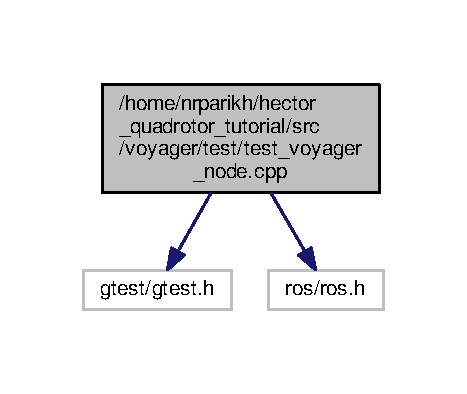
\includegraphics[width=224pt]{test__voyager__node_8cpp__incl}
\end{center}
\end{figure}
\subsection*{Functions}
\begin{DoxyCompactItemize}
\item 
int \hyperlink{test__voyager__node_8cpp_a3c04138a5bfe5d72780bb7e82a18e627}{main} (int argc, char $\ast$$\ast$argv)
\begin{DoxyCompactList}\small\item\em Run all the unit tests. \end{DoxyCompactList}\end{DoxyCompactItemize}


\subsection{Detailed Description}
D\+E\+S\+C\+R\+I\+P\+T\+I\+ON Unit tests for the package Voyager. 

\begin{DoxyAuthor}{Author}
nr-\/parikh 
\end{DoxyAuthor}
\begin{DoxyCopyright}{Copyright}
M\+IT license (c) 2017 Neel Parikh 
\end{DoxyCopyright}


\subsection{Function Documentation}
\index{test\+\_\+voyager\+\_\+node.\+cpp@{test\+\_\+voyager\+\_\+node.\+cpp}!main@{main}}
\index{main@{main}!test\+\_\+voyager\+\_\+node.\+cpp@{test\+\_\+voyager\+\_\+node.\+cpp}}
\subsubsection[{\texorpdfstring{main(int argc, char $\ast$$\ast$argv)}{main(int argc, char **argv)}}]{\setlength{\rightskip}{0pt plus 5cm}int main (
\begin{DoxyParamCaption}
\item[{int}]{argc, }
\item[{char $\ast$$\ast$}]{argv}
\end{DoxyParamCaption}
)}\hypertarget{test__voyager__node_8cpp_a3c04138a5bfe5d72780bb7e82a18e627}{}\label{test__voyager__node_8cpp_a3c04138a5bfe5d72780bb7e82a18e627}


Run all the unit tests. 

Running all the tests for all the classes


\begin{DoxyParams}{Parameters}
{\em argc} & Number of arguments passed \\
\hline
{\em argv} & Array for passed arguments\\
\hline
\end{DoxyParams}
\begin{DoxyReturn}{Returns}
0 if all the tests are passed 
\end{DoxyReturn}


Definition at line 45 of file test\+\_\+voyager\+\_\+node.\+cpp.


%--- End generated contents ---

% Index
\backmatter
\newpage
\phantomsection
\clearemptydoublepage
\addcontentsline{toc}{chapter}{Index}
\printindex

\end{document}
